{
\chapter[Global visual salience of competing stimuli]{Global visual salience\\of competing stimuli}
\label{ch:globsal}
\renewcommand{\chapterpath}{includes/global-salience}
%
\begin{contributors}
    Ricardo Ramos Gameiro designed the first prototype of the experiments, collected the eye tracking data and contributed to the original draft of the manuscript. Alessandro Grillini contributed to the comparisons between global and local salience and to the corresponding part of the original draft. Peter K{\"o}nig contributed to the conceptualisation of the project and supervised the work. Ricardo, Alessandro and Peter reviewed and edited the manuscript submitted to the Journal of Vision.
\end{contributors}
%
\begin{outreach}
    \item \textit{Global visual salience of competing stimuli.} \textbf{Alex Hern{\'a}ndez-Garc{\'i}a}, Ricardo Ramos Gameiro, Alessandro Grillini, Peter K{\"o}nig. PsyArXiv preprint PsyArXiv:z7qp5 \& Journal of Vision (accepted), 2019.
\end{outreach}
%
Visual attention is a highly complex mechanism that facilitates our understanding and navigation of the world around us, by enabling the coherent processing of the large amount of information that enters our eyes. Therefore, a fundamental component of vision and hence cognition is the guidance of eye movements \citep{liversedge2000eyemovements, geisler2011eyemovements, konig2016eyemovements}. We constantly have to decide where to look next and which regions of interest to explore, in order to process and interpret relevant information of a scene. As a consequence, the investigation of eye movement behaviour has become a major field in many research areas \citep{kowler2011eyemovements, kaspar2013visualattention}. 

In this regard, a number of studies have shown that visual behaviour is controlled by three major mechanisms: bottom-up, top-down, and spatial biases \citep{desimone1995visualattention, egeth1997visualattention, kastner2000visualattention, corbetta2002topdownbottomup, connor2004buttomuptopdown, kollmorgen2010topdownbottomup}. Bottom-up factors describe features of the observed image, which attract eye fixations, involving primary contrasts, such as colour, luminance, brightness, and saturation \citep{itti1998salience, reinagel1999bottomup, baddeley2006bottomup}. Hence, bottom-up factors are typically based on the sensory input. In contrast, top-down factors comprise internal states of the observer \citep{connor2004buttomuptopdown, kaspar2013visualattention}. That is, eye movement behaviour is also guided by specific characteristics, such as personal motivation, specific search tasks, and emotions \citep{wadlinger2006topdown, einhauser2008topdown, rauthmann2012topdown, kaspar2012topdown}. Finally, spatial properties of the image, such as the image size, and motor constraints of the visual system in the brain may affect eye movement behaviour \citep{ramosgameiro2017explorationexploitation, ossandon2014spatialbiases}. As a result, spatial properties and motor constraints then lead to specific bias effects, such as the central bias in natural static images \citep{tatler2007centralbias}. Thus, investigating visual behaviour necessarily implies an examination of bottom-up and top-down factors as well as spatial biases. 

Based on these three mechanisms---bottom-up, top-down and spatial biases---guiding visual behaviour, \citet{koch1987salience} first revealed a method to highlight salient points in static image scenes. Whereas this model was purely conceptual, \citet{niebur1996salience} later developed an actual implementation of salience maps. This was the first prominent proposal of topographically organised features maps that guide visual attention. Salience maps describe these topographic representations of an image scene, revealing where people will most likely look at while observing the respective scene \citep{itti2001salience}. That is, salience maps can be interpreted as a prediction of the distribution of eye movements on images. Usually, salience maps include only bottom-up image features, predicting eye fixations on image regions with primary contrasts in colour changes, saturation, luminance or brightness among others \citep{itti1998salience}. However, in their first implementation, \citet{niebur1996salience} also tried to include top-down factors to build up salience maps and thus predict where people will look at most likely in image scenes. Current state-of-the-art computational salience models are artificial neural networks pre-trained on large data sets for visual object recognition and subsequently tuned to predict fixations, as is the case of Deep Gaze II \citep{kuemmerer2016deepgaze}. Such models do not rely only on bottom-up features any more, but also incorporate higher-level features learned on object recognition tasks. Still, despite the better performance on salience benchmarks, deep nets-based models seem to fail at predicting the salience driven by low-level features \citep{kuemmerer2017icfdeepgaze}.

Salience maps provide a highly accurate and robust method to predict human eye movement behaviour on static images, by relying on local features to determine which parts of an image are most salient \citep{niebur1996salience, itti2001salience, kowler2011eyemovements}. However, these methods do not provide any information about the salience of the image as whole, which may depend on both local properties and also the overall semantic and contextual information of the image. Such global salience is of great relevance when an observer is faced with two or more independent visual stimuli in one context. These combinations describe situations when several stimuli compete with each other with regard to their individual semantic content, despite being in the same overall context. Such cases appear frequently in real life, for instance when two billboards hang next to each other in a mall, when several windows are open on a computer screen, or a monitor on intensive care unit, to name a few examples. Thus, by placing two or more independent image contexts side by side, as described in the previous examples, classical salience maps may well predict eye movement behaviour within each of the individual images as a closed system, but they will most likely fail to predict visual behaviour across the whole scene involving all images. Specifically, they will fail at answering the question: which stimulus is most likely to attract the observers' visual attention?

\section{Hypotheses and contributions}
\label{sec:globsal-contributions}
In this chapter, we present the work of a study where we postulate several hypotheses. Our primary hypothesis (H1) is that it is possible to measure and calculate the global salience of natural images. That is, the likelihood of a visual stimulus to attract the first fixation of a human observer, when it is presented in competition alongside another stimulus, can be systematically modelled. In the experiment presented here, participants were confronted with stimuli containing two individual natural images---one on the left and one on the right side of the screen---at the same time. The set of images used to build our stimuli consisted of urban, indoor and nature scenes, close-ups of human faces and scenes with people in a social context. During the observation of the image pairs, we recorded the participants' eye movements. Specifically, to characterise the global salience we were interested in the direction---left or right---of the initial saccade the participant made after the stimulus onset. For further analysis, we also collected all binary saccade decisions on all the image pairs presented to the participants. We used the behavioural data collected from the participants to train a logistic regression model that successfully predicts the location of the first fixation for a given pair of images. This allowed us to use the coefficients of the model to characterise the likelihood of each image to attract the first fixation, relative to the other images in the set. In general, images that were fixated more often are ranked higher than other images. Hence, we computed a unique \textit{attraction score} for each image that we denote \textit{global salience}, which depends on the individual contextual information of the image as a whole. 

We also analysed the local salience properties of the individual images and compared it to the global salience. We hereby claimed that the global salience cannot be explained by the feature-driven salience maps. Formally, we hypothesise that (H2): Natural images have a specific global salience, independent of their local salience properties, that characterises their likelihood to attract the first fixation of human observers, when presented alongside another competing stimulus. A larger global salience leads to a higher attraction of initial eye movements.  

In order to properly calculate the global salience, we accounted for general effects of visual behaviour in stimuli with two paired images. Previous studies have shown that humans tend to exhibit a left bias in scanning visual stimuli. \citet{barton2006leftbias} showed that subjects looking at faces fixated longer the eye on their left side, even if the faces were inverted, and the effect was later confirmed and extended to dogs and monkeys \citep{guo2009leftbias}. For an extensive review about spatial biases see the work by \citet{ossandon2014spatialbiases}, where the authors presented evidence of a marked initial left bias in right-handers, but not in left-handers, regardless of their habitual reading direction. In sum, there is a large body of evidence of lateral asymmetry in viewing behaviour, although the specific sources are yet to be fully confirmed. With respect to our study, we hypothesise that (H3): Presenting images in horizontal pairs leads to a general spatial bias in favour of the image on the left side. 

In addition to the general left bias, in half of the trials of the experimental sessions, one of the images had been already seen by the participant in a previous trial, while the other was new. The participants also had to indicate which of the images was new or old. Thus, we also addressed the questions of whether the familiarity with one of the images or the task have any effect in the visual behaviour and thus in the global salience of the images. Do images that show the task-relevant scene attract more initial saccades? Likewise, are novel images more likely to attract the first fixation? This challenge sheds some light on central-peripheral interaction in visual processing. \citet{guo2007topdown}, for instance, showed that during face-processing, humans indeed rely on top-down information in scanning images. However, \citet{acik2010bottomuptopdown} proposed that young adults usually rely on bottom-up rather than top-down information during visual search. In this regard, we thus hypothesise that (H4): Task-relevance and familiarity of images will not lead to higher probability of being fixated first. In order to account for any spatial bias effects that could influence the global salience model, we added coefficients to the logistic regression algorithm that could potentially capture any lateral, familiarity and bias effects. This not only makes the model more accurate, but allows us to analyse the influence of these effects. Furthermore, the location of the images in the experiments was randomised across trials and participants. 

Finally, in order to better understand the properties of the global salience of competing stimuli, we also analysed the exploration time of each image. In this regard, we hypothesise the following (H5): Images with larger global salience will be explored longer than images with low global salience.

\section{Methods: experimental setup}
\label{sec:globsal-methods}
The present study was conducted in the Neurobiopsychology lab at the Institute of Cognitive Science of the University of Osnabr\"uck, Germany. The experimental methods were approved by the Ethical Committee of the University of Osnabr\"uck, Germany, and performed in accordance with the guidelines of the German Psychological Society. All participants gave written consent to participate in this study. 

\subsection{Participants}
\label{sec:globsal-methods_participants}
Forty-nine healthy participants (33 females, mean age = 22.39 years, \textit{SD} = 3.63) with normal or corrected-to-normal vision took part in this study. All participants were instructed to freely observe the stimuli on the screen. In part of the measurements, they had to indicate after the trial the old or new image of a pair as further described below.  

\subsection{Apparatuses}
\label{sec:globsal-methods_apparatuses}
We presented the stimuli on a 32'' widescreen Samsung monitor (Apple, California, USA) with a native resolution of 3840 $\times$ 2160 pixels. For eye movement recordings, we used a stationary Eye Link 1000 eye tracker (SR Research Ltd.) providing binocular recordings with one head camera and two eye cameras with sampling rate of 500 Hz.

Participants were seated in a darkened room at a distance of 80 cm from the monitor, resulting in 80.4 pixels per visual degree in the centre of the monitor. We did not fixate the participant's head with a headrest but verbally instructed the participants not to make head movements during the experiment. This facilitated comfortable conditions for the participants. However, eye tracker constantly recorded four edge markers on the screen with the head camera, in order to correct for small head movements. This guaranteed stable gaze recordings based on eye movements, independent of residual involuntary head movements. 

The eye tracker measured binocular eye movements. For calibration of the eye tracking camera, each participant had to fixate on 13 black circles (size 0.5\textdegree) that appeared consecutively at different screen locations. The calibration was validated afterwards by calculating the drift error for each point. The calibration was repeated until the system reached an average accuracy of \textless~0.5\textdegree\ for both eyes of the participant.

\subsection{Stimuli}
\label{sec:globsal-methods_stimuli}
The images set consisted of 200 images, of which 197 were natural photographs and 3 were randomly generated pink noise images. Altogether, the stimulus set was divided into 6 categories, according to the image content: human faces, urban scenes, natural landscapes, indoor scenes, social activities and pink noise. All the photographs were obtained from either the internal image database of the Neurobiopsychology laboratory at the University of Osnabr\"uck, Germany or the NimStim database. Each image was scaled to a resolution of 1800 $\times$ 1440 pixels. Some examples are shown in Figure~\ref{fig:globsal-stimuli_samples}.

Each trial consisted of one stimulus with a resolution of 3840 $\times$ 2160 pixels, matching the full-size screen resolution of the display monitor (32'' diagonal; 47.8\textdegree\ $\times$ 26.9\textdegree). Within each presented stimulus, two images were randomly paired that is, one image was shown on the left screen side and the other image on the right screen side. Between both images, each stimulus contained a central gap of 240 pixels, as illustrated by Figure~\ref{fig:globsal-stimuli_pair}. The background area of the stimuli was set to middle grey.

\begin{figure}[ht]
  \centering
  \begin{subfigure}{0.48 \linewidth}
      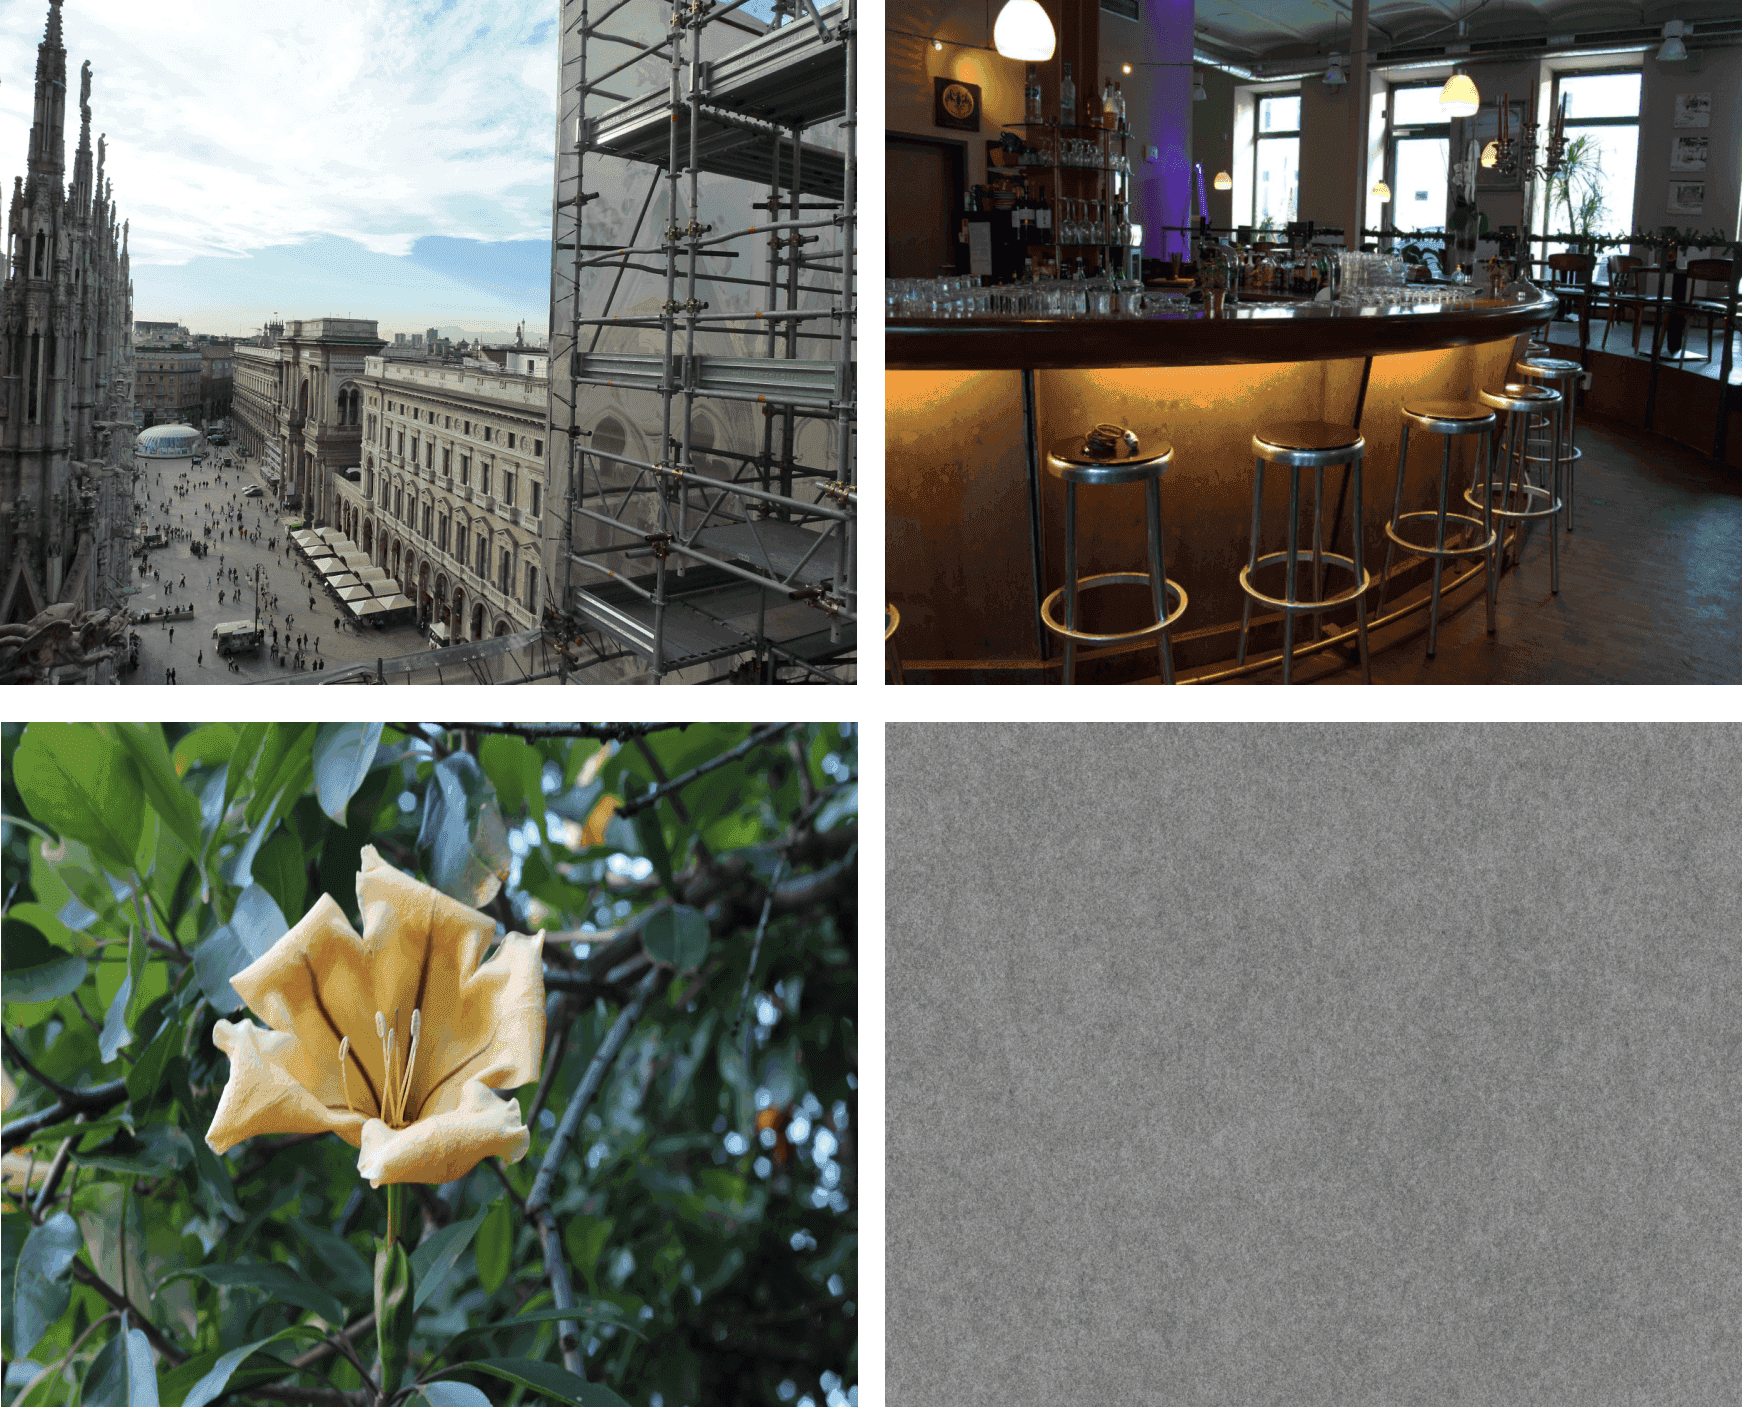
\includegraphics[width = \linewidth]{\imgpath/stimuli_samples.png}
      \caption{Four images from the set}
    \label{fig:globsal-stimuli_samples}
  \end{subfigure}
  \hspace{0.02 \linewidth}
  \begin{subfigure}{0.48 \linewidth}
      \centering
      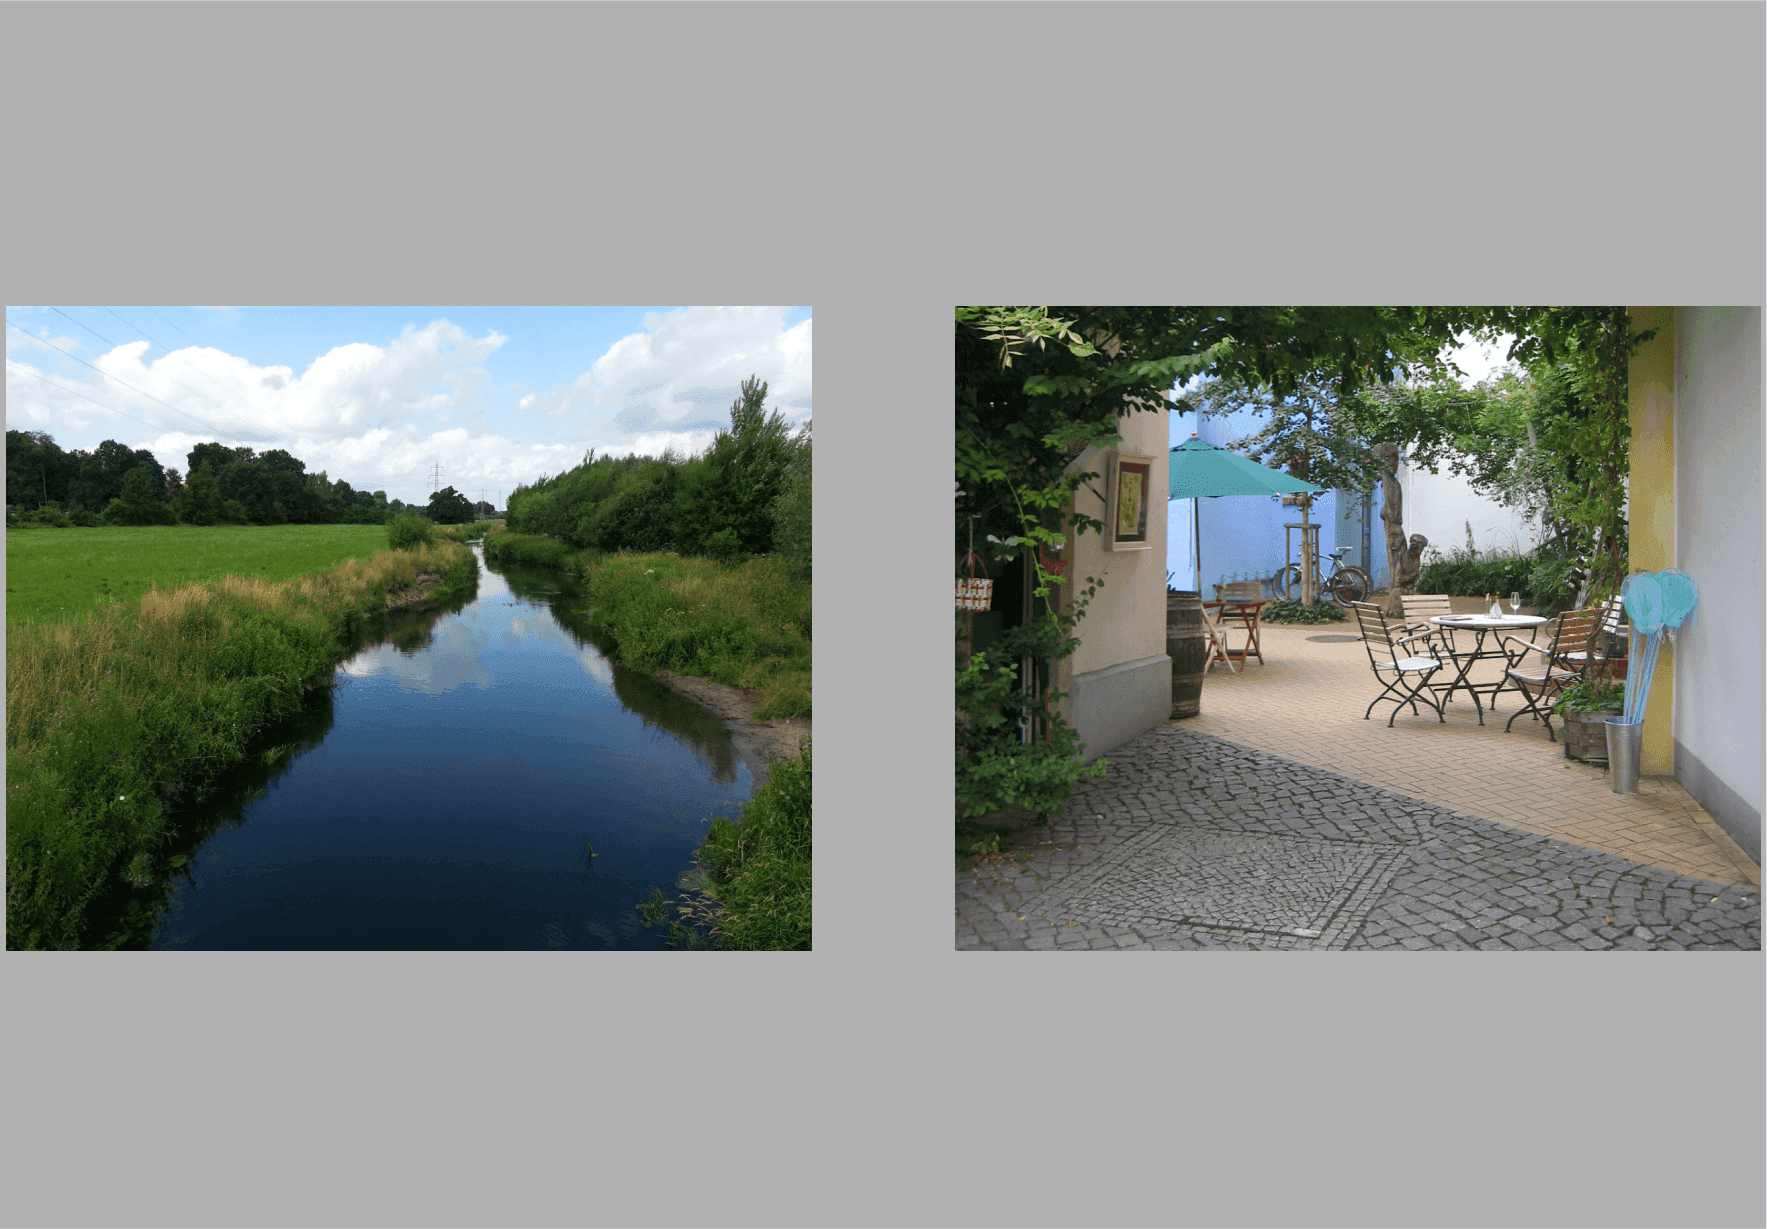
\includegraphics[width = \linewidth]{\imgpath/stimuli_pair.png}
      \caption{The stimulus at one trial}
    \label{fig:globsal-stimuli_pair}
  \end{subfigure}
  \\
  \begin{subfigure}{0.43 \linewidth}
      \centering
      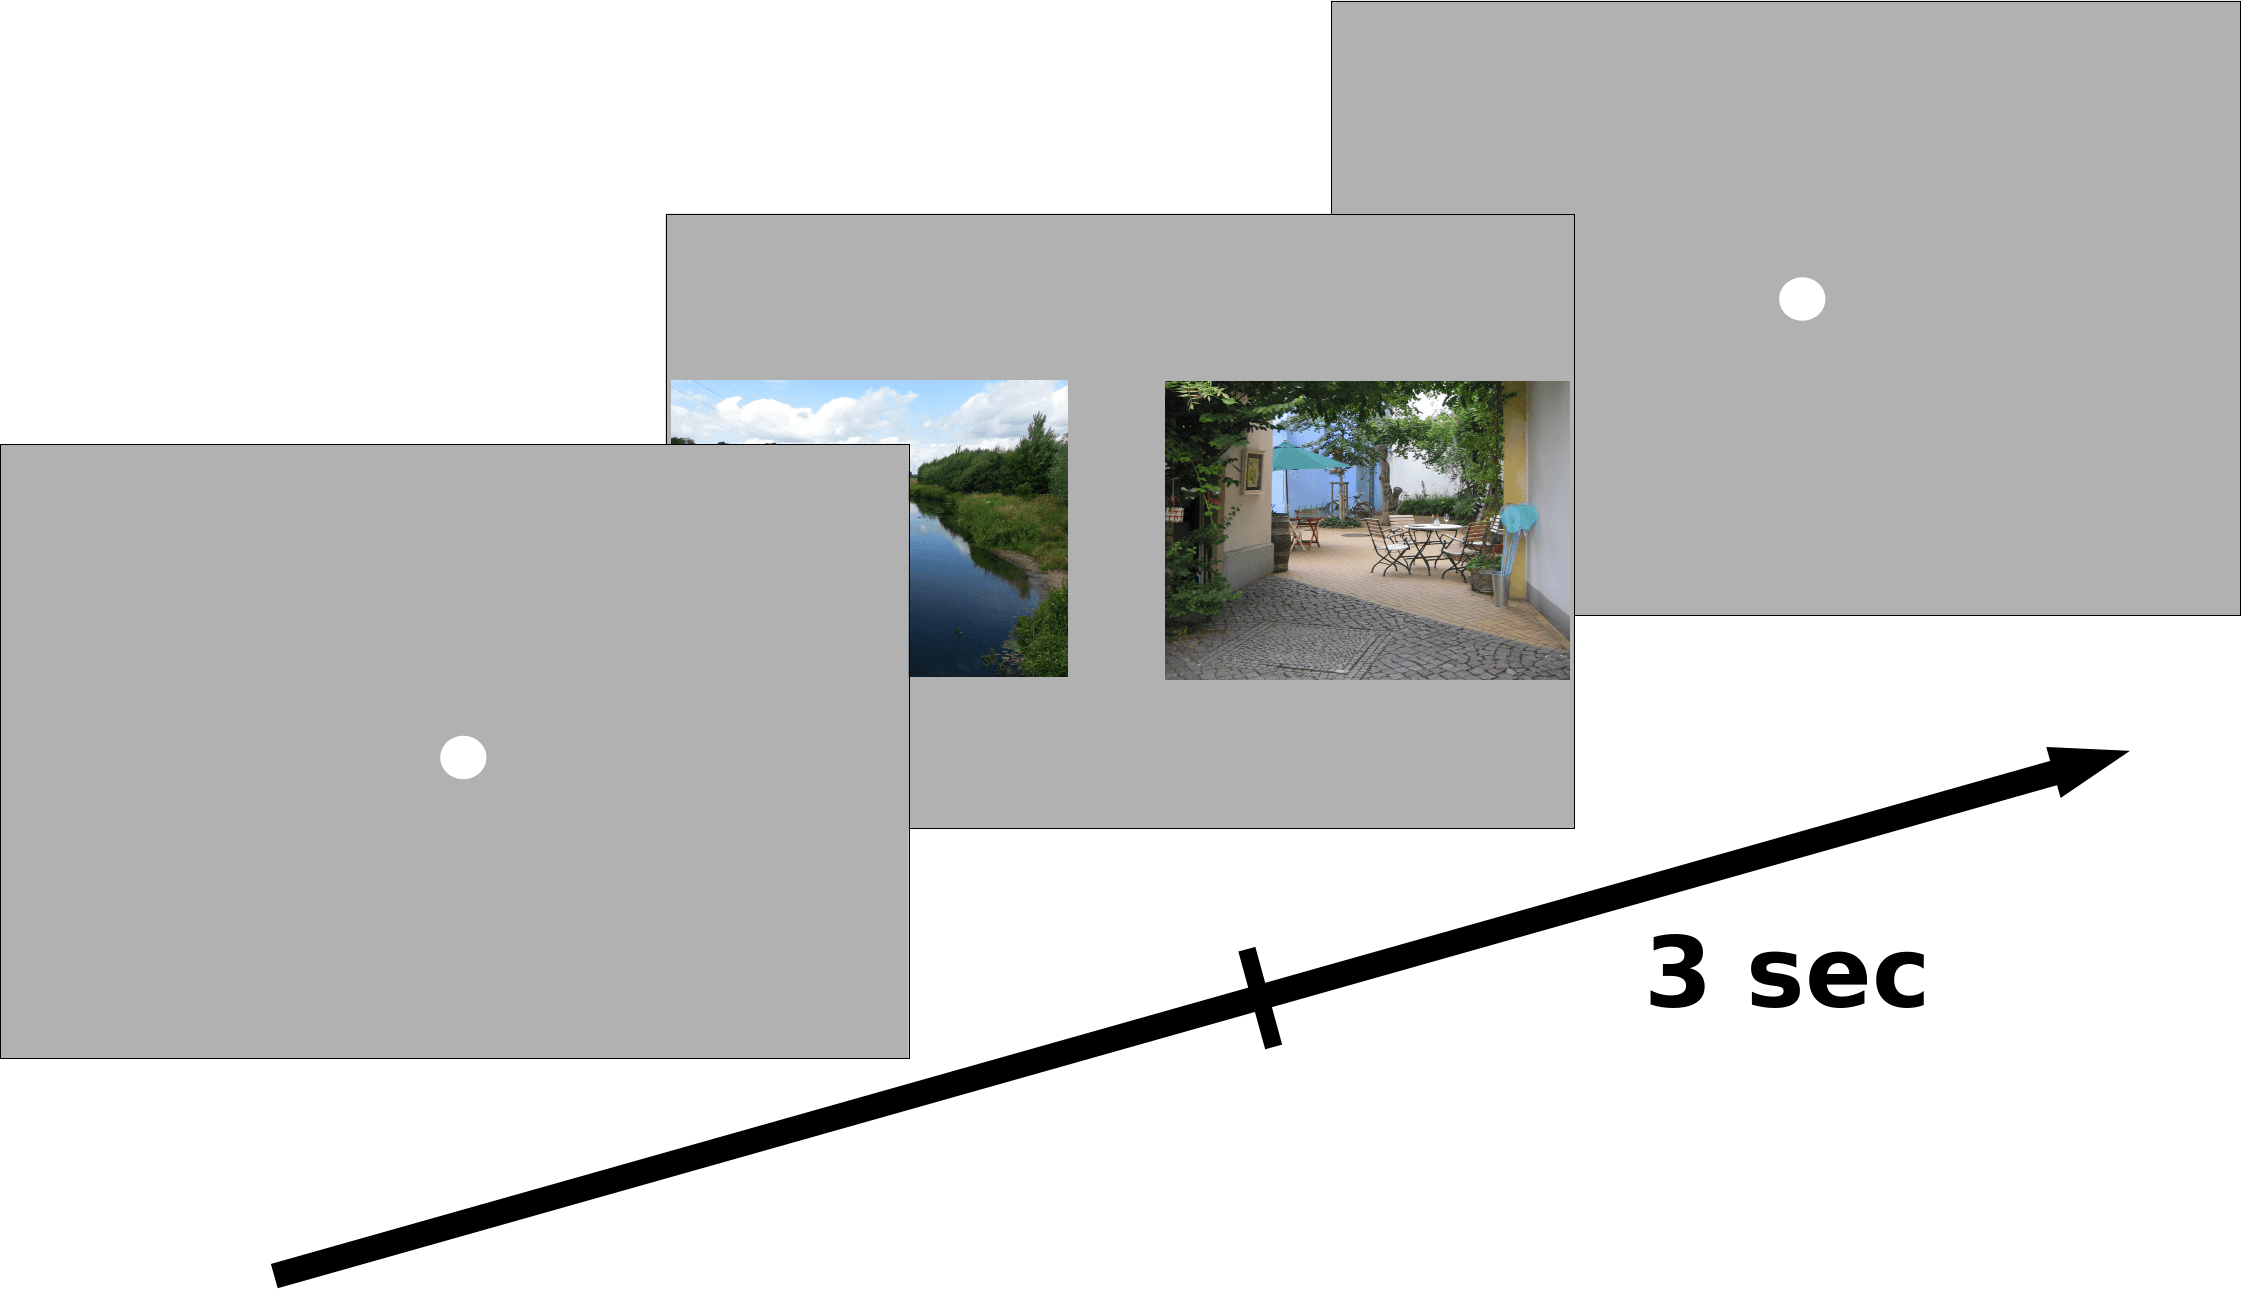
\includegraphics[width = \linewidth]{\imgpath/trial_notask.png}
      \caption{Procedure in blocks 1 and 4, where no task was given}
    \label{fig:globsal-trial_notask}
  \end{subfigure}
  \hspace{0.02 \linewidth}
  \begin{subfigure}{0.53 \linewidth}
      \centering
      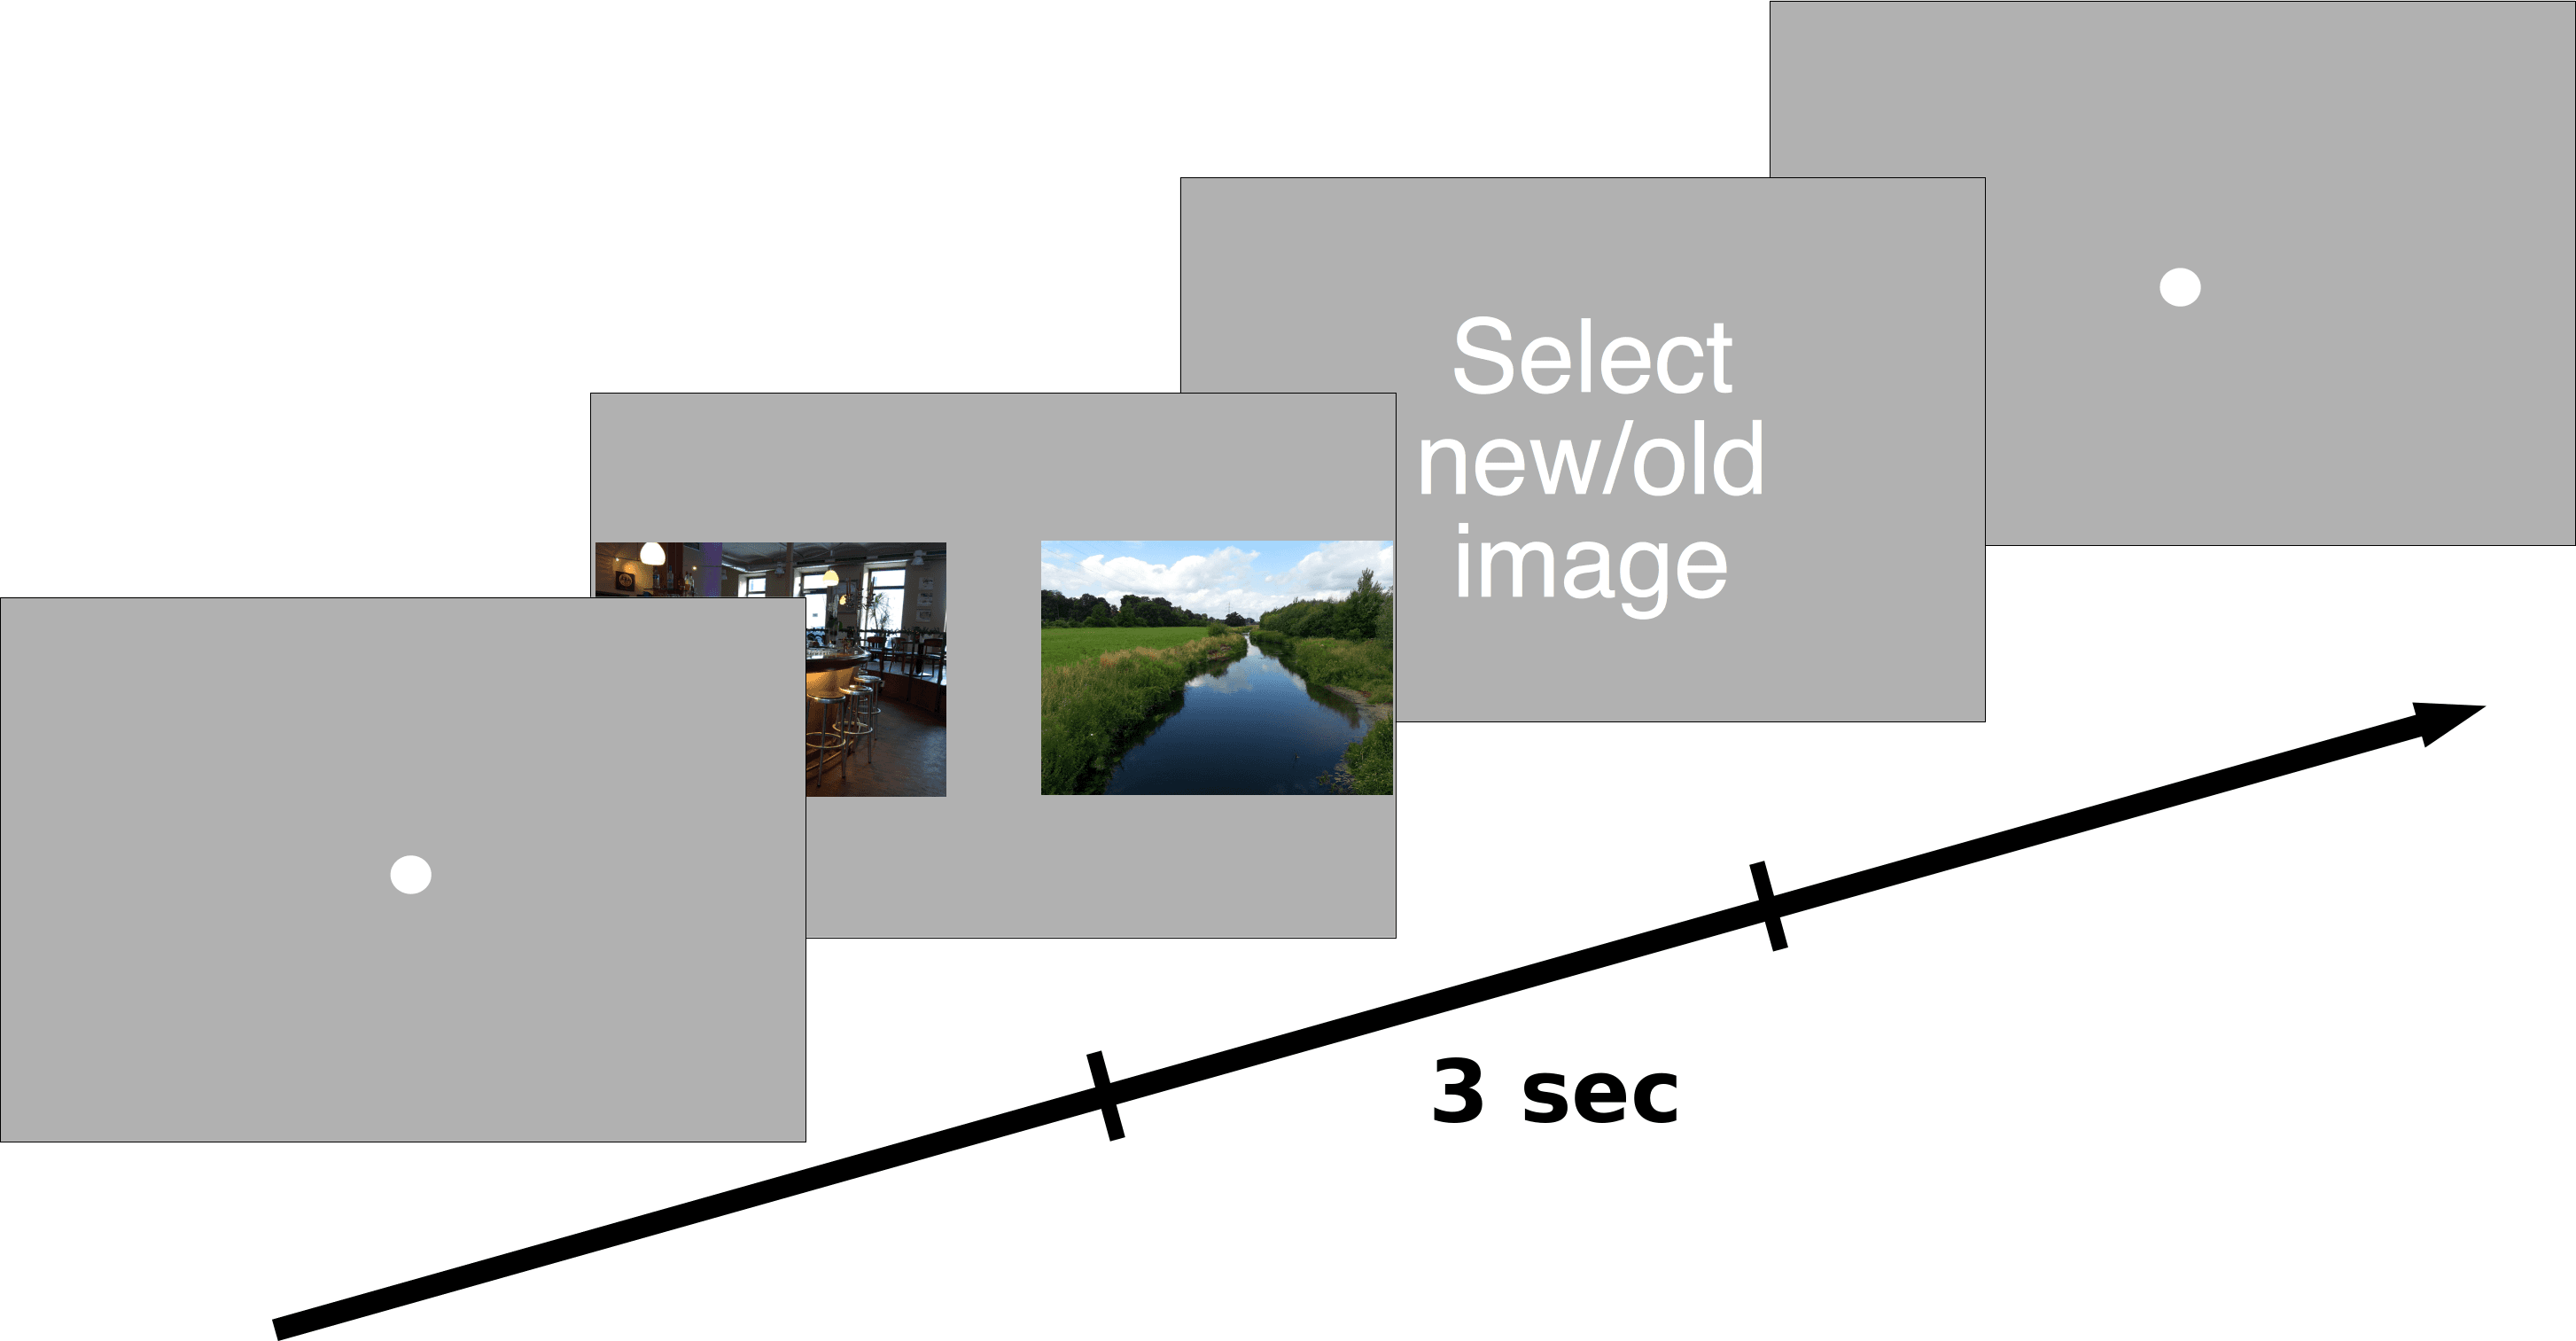
\includegraphics[width = \linewidth]{\imgpath/trial_task.png}
      \caption{Procedure in blocks 2 and 3, where participants had to perform a simple task after the stimulus offset}
    \label{fig:globsal-trial_task}
  \end{subfigure}
  \caption{Experimental setup}
\label{fig:globsal-experiment}
\end{figure}

\subsection{Procedure}
\label{sec:globsal-methods_procedure}

The experiment consisted of 200 trials divided into four blocks, at the beginning of which the eye-tracking system was re-calibrated. The blocks were designed such that each had a different combination of task and image novelty:

\begin{itemize}
    \item \textbf{Block 1} consisted of 25 trials formed by 50 distinct, novel images (new/new). This block was task-free, that is participants were guided to freely observe the stimuli (Figure~\ref{fig:globsal-trial_notask}).
    \item \textbf{Block 2} consisted of 75 trials, each formed by one new image and one of the previously seen images. (new/old or old/new). In this block, the participants were guided to freely observe the stimuli and, additionally, they were asked to indicate the \textit{new} image of the pair after the stimulus offset (Figure~\ref{fig:globsal-trial_task}).
    \item \textbf{Block 3} consisted of 75 trials, each formed by one new image and one of the previously seen images. (new/old or old/new). In this block, the participants were asked to indicate the \textit{old} image of the pair.
    \item \textbf{Block 4} consisted of 25 trials formed by 50 previously seen images (old/old). Like block 1, this block was also task-free.
\end{itemize}

The decision in blocks 2 and 3 was indicated by either pressing the left---task-relevant image is on the left side---or right---task relevant-image is on the right side---arrow button on a computer keyboard. 

The image pairs were formed by randomly sampling from the set of 200 images, but some constraints were set in order to satisfy the characteristics of each block and keep a balance in the number of times each image was seen by the participant. The sampling process was as follows: In block 1, 50 images were randomly sampled to form the 25 pairs. In blocks 2 and 3, in order to construct the new/old and old/new pairs, the new image was randomly sampled from the set of remaining unseen images and the old image was randomly sampled of previously seen images, with two additional constraints: it must have been chosen only one time before and not in the previous 5 trials. Finally, in block 4, a set of exactly 50 images which had been shown only once remained. These were used to randomly sample the remaining 25 trials. In all blocks, after sampling the two images, the left/right configuration was also randomly chosen with probability 0.5.
    
The sampling process was different for each participant, that is they saw different sets of pairs from the 40,000 different pairs and in different order. This aimed at reducing the predictability of the process while satisfying the experimental constraints. Overall, we collected data from 9,800 pairs, some of which might have been repeated across participants. However, note that each participant saw each image exactly twice, therefore the frequency of presentation of the images was balanced across the whole experiment. As we will see in the following section, the amount of data was enough to fit the computational model. 

In all cases, the presentation time for each stimulus was 3 seconds and it was always preceded by a blank, grey screen with a white, central fixation dot. The stimulus was displayed only after the participant fixated the central dot. 

The majority of our analyses focused on the first fixation. As a pre-processing stage, we discarded the fixations 1) due to anticipatory saccades, 2) shorter than 50 ms or longer than $\mu_{dur} + 2 \sigma_{dur}$ ms, where $\mu_{dur} = 198$ ms and $\sigma_{dur} = 90$ ms are the mean and standard deviation of all fixation durations, respectively, and 3) located outside any of the two images. The discarded fixations were less than 4~\% of the total.

\section{Methods: computation of global salience}
\label{sec:globsal}
In order to characterise the global salience of competing stimuli, we trained a logistic regression model with the behavioural data from the eye-tracking experiments. Provided that the model can accurately predict the location of the first fixation---left or right---the coefficients for each image will represent the likelihood of the image to attract the first fixation and this, in turn, can then be interpreted as the global image salience. The intuition is that images that are more often the target of the first fixation after the stimulus onset have a higher global salience, and vice versa.

\subsection{Logistic regression for pairwise estimates}
\label{sec:globsal-logreg_plain}
Typically, logistic regression is used in binary classification problems, as is this case where the initial fixation after stimulus onset can land either on the left ($y = -1$) or on the right ($y = 1$) image. The classifier simply estimates a probability $h_{w}(\mathbf{x})$ for the binary event on the linear hypothesis $\mathbf{w}^{T}\mathbf{x}$ by applying a logistic function:

\begin{equation}
\label{eq:logreg}
 h_{w}(\mathbf{x}) = \frac{1}{1 + e^{-\mathbf{w}^{T}\mathbf{x}}} = \frac{e^{\mathbf{w}^{T}\mathbf{x}}}{1 + e^{\mathbf{w}^{T}\mathbf{x}}}
\end{equation}
%
where $\mathbf{x}$ is a vector that represents the independent or explanatory variables (features) and $\mathbf{w}$ the coefficients to be learned. Thus, the likelihood of the binary outcome given the data is the following:

\[   
P(y|\mathbf{x}) = 
     \begin{cases}
       h_{w}(\mathbf{x})  &\quad\text{if } y = 1\\
       1 - h_{w}(\mathbf{x})  &\quad\text{if } y = -1\\
     \end{cases}
= \frac{e^{y\mathbf{w}^{T}\mathbf{x}}}{1 + e^{y\mathbf{w}^{T}\mathbf{x}}}
\]

The coefficients are then optimised by minimising the negative log-likelihood $-log(P(y|\mathbf{x}))$ through gradient descent. Typically, a regularisation penalty is added on the coefficients, controlled by the parameter $C$---inverse of the regularisation strength. In our case, we applied $L_2$ regularisation and therefore the algorithm solves the following optimisation problem, given a set of $N$ training data points (trials):

\begin{equation}
\label{eq:objective}
\min_{\mathbf{w}} \frac{1}{2}\mathbf{w}^{T}\mathbf{w} + C\sum_{i=1}^{N}log(1 + e^{-y_{i}\mathbf{w}^{T}\mathbf{x}_{i}})
\end{equation}

The optimisation problem was solved through the \textit{LIBLINEAR} algorithm \citep{fan2008liblinear}, available in the \texttt{scikit-learn} Python toolbox.

In our particular case, for every trial $i$---stimulus pair seen by a participant---each feature $x_{ij}$ corresponded to one image $j$ and only two images were shown at each trial. Therefore, we were interested in modelling the probability that one image $u$ receives the first fixation when presented next to another image $v$; hence $p(u > v)$. This simplifies the standard logistic regression model to a special case for pairwise probability estimates, known as the Bradley-Terry-Luce model \citep{bradley1952pairwisecomp, luce2005pairwisecomp}, where the probability $h_{w}$ is the following:

\begin{equation}
\label{eq:btl}
 h_{w}(u,v) = p(u > v) = \frac{e^{w_{u}}}{e^{w_{u}} + e^{w_{v}}} = \frac{e^{w_{u}-w_{v}}}{1 + e^{w_{u}-w_{v}}}
\end{equation}
%
where $w_{u}$ and $w_{v}$ are the coefficients of image $u$ and $v$. This is a special case of the function in Equation \ref{eq:logreg}, where all the elements in the feature vector $\mathbf{x}$ are zero except for the two paired features $x_{u}$ and $x_{v}$, which are set to 1 and -1 respectively. Note that in the Bradley-Terry-Luce model the coefficients still refer to the whole set of features and therefore are described by an $M$-dimensional vector $\mathbf{w} = \{w_{1}, w_{2}, ..., w_{M}\}$, where in our case $M=200$, the total number of images in the set. After training the model, each learned coefficient $w_{j}$ will be related to the average likelihood of image $j$ of receiving the first fixation when presented next to other images from the set. As stated above, we interpret these coefficients $\mathbf{w}$ as a measure of the global image salience.

In order to estimate the coefficients $\mathbf{w}$, the logistic regression model was trained on the data set arranged into a design matrix $X$ of the following form:

\begin{equation}
\label{eq:matrix_x}
X = 
\begin{bmatrix}
    x_{1}^{(1)} & x_{2}^{(1)} & \dots  & x_{M}^{(1)} \\
    x_{1}^{(2)} & x_{2}^{(2)} & \dots  & x_{M}^{(2)} \\
    \vdots      & \vdots      & \ddots & \vdots      \\
    x_{1}^{(N)} & x_{2}^{(N)} & \dots  & x_{M}^{(N)} \\
\end{bmatrix}
\end{equation}
%
where each row represents one measured data point: one trial where one participant was presented a pair of images $u$ and $v$---the total number of trials was in our case $N = 49~\text{participants} \times 200~\text{trials per participant} = 9800$---and where the columns represent the values of the different features (images) that were tested ($M = 200$). According to Equation~\ref{eq:btl}, if image $u$ is presented on the right and image $v$ is presented on the left at trial $i$, then $x_{u}^{(i)}=1$, $x_{v}^{(i)}=-1$ and $x_{j}^{(i)}=0, \forall~j \neq u,v$. Finally, the outcome of each trial is given as a vector $\mathbf{y}$:

\[
\mathbf{y} =
\begin{bmatrix}
    y^{(1)} \\
    y^{(2)} \\
    \vdots  \\
    y^{(N)} \\
\end{bmatrix}
\]
%
such that $y^{(i)} = 1$ if the right image was fixated first, and $y^{(i)} = -1$ if the left image was fixated first at trial $i$. 

\subsection{Task, familiarity and lateral bias} 
\label{sec:globsal-biases}
Not only were we interested in modelling the likelihood of every image of receiving the first fixation, but also the contribution of other aspects of the experiment, namely the effect of having to perform a small task when observing the pair of images and the familiarity with one of the two images. More specifically, we were interested in answering the following questions: Do light task demands, such as having to determine  which image is new or old, influence the direction of the first saccade? And, are unseen stimuli more likely to receive the initial saccade than previously observed stimuli when presented together, or vice versa?

We addressed these questions by adding new features to the model that capture these characteristics of the experimental setup. These features were assigned coefficients that, after training, will indicate the magnitude of the contributions of the effects. In particular, we added the following features columns to every row $i$ of the design matrix:

\begin{itemize}
 \item $t^{(i)}$: 1 if the target of the task (select new/old image) was on the right at trial $i$, -1  image if on the left, 0 if no task.
 \item $f^{(i)}$: 1 if at trial $i$, the image on the right had been already shown at a previous trial (familiar), while the image on the left was still unseen; -1 if the familiar image was on the left; 0 if both images were new or familiar.
\end{itemize}

Not only did these new features enable new elements for the analysis, but also added more representational power to the model, which could potentially learn better coefficients to describe the global salience of each image. In this line, we added one more feature to the model to capture one important aspect of visual exploration: the lateral bias. Although a single intercept term in the argument of the logistic function ($\mathbf{w}^{T}\mathbf{x} + b)$ would capture most of the lateral bias, since the outcome $\mathbf{y}$ describes exactly the lateral direction, left or right, of the first saccade, we instead added subject-specific features to model the fact that the trials were generated by different subjects with an individual lateral bias. This was done by adding $K = 49$ (number of participants) features $s_{k}^{(i)}$, with value 1 if the trial $i$ was performed by subject $k$ and 0 otherwise. Altogether, the final design matrix $X^{\prime}$ extends the design matrix $X$ defined in Equation~\ref{eq:matrix_x} as follows:

\begin{equation}
\label{eq:matrix_x_prime}
X^{\prime} = 
\begin{bmatrix}[ccc|c|c|ccc]
    x_{1}^{(1)} & \dots  & x_{M}^{(1)} & t^{(1)} & f^{(1)} & s_{1}^{(1)} & \dots  & s_{K}^{(1)} \\
    x_{1}^{(2)} & \dots  & x_{M}^{(2)} & t^{(2)} & f^{(2)} & s_{1}^{(2)} & \dots  & s_{K}^{(2)} \\
    \vdots      & \ddots & \vdots      & \vdots  & \vdots  & \vdots      & \ddots & \vdots      \\
    x_{1}^{(N)} & \dots  & x_{M}^{(N)} & t^{(N)} & f^{(N)} & s_{1}^{(N)} & \dots  & s_{K}^{(N)} \\
\end{bmatrix}
\end{equation}

Note that the leftmost block of $X^{\prime}$ is identical to $X$ (defined in Equation~\ref{eq:matrix_x}). While the shape of $X$ is $9800 \times 200$, $X^{\prime}$ is a $9800 \times 251$ matrix, since $200 + 1 + 1 + 49 = 251$.

\subsection{Validation and evaluation of the model} 
\label{sec:globsal-model_eval}
In order to ensure the successful training of the model, we carried out a 5-fold cross-validation of the regularisation parameter $C$ of the model, described in Equation~\ref{eq:objective}. That is, we split our data set into 5 different folds of 39 subjects for training and 10 for validation---7,800 and 2,000 trials, respectively---and evaluated the performance with 10 different values of $C$, according to the following search space:

\[C = 10^{p} \quad\text{with}~p = -3 + \frac{2}{3}(n-1) \quad\text{and}~n=1, ..., 10 \]

The value that provided the best average performance across the folds was selected.

In order to reliably assess the model performance while taking the most out of the data set, we embedded the cross-validated model into a \textit{leave-2-participants-out} cross-evaluation. That is, we constructed 25 different folds of data, each with the trials of 23 participants for training and of 2 participants for evaluation. We report here the average performance across the 25 test and train partitions together with the standard deviation (within brackets). In particular, in Table \ref{tab:performance} we include the area under the curve (AUC), the Tjur\footnote{While there is no consensus about the best metric for the evaluation of logistic regression, the coefficient of discrimination $R^{2}$ proposed by \citet{tjur2009r2} has been widely adopted recently, as it is more intuitive than other definitions of coefficients of determination and still asymptotically related to them.} coefficient of discrimination $R^{2}$ and the accuracy. For the sake of an easier interpretation, we include the theoretical baseline values of the AUC and $R^{2}$, and the empirical baseline accuracy on our test partitions.

\begin{table}[ht]
\centering
  \begin{tabular}{rccc}
    \multicolumn{1}{l}{} & AUC             & Tjur $R^{2}$         & Accuracy        \\
    \hline \\
    Test                 & 0.8884 (0.0180) & 0.4287 (0.0460) & 81.36 \% (0.32) \\
    Train                & 0.8865 (0.0040) & 0.4240 (0.0214) & 81.99 \% (1.52) \\
    Random baseline      & 0.5             & 0.0             & 60.70 \% (2.32)
  \end{tabular}
\caption{Test, train and baseline performance of the logistic regression model. Values within brackets indicate the standard deviation across the folds.}
\label{tab:performance}
\end{table}

The results in Table~\ref{tab:performance} show that the logistic regression model successfully learned the behavioural patterns from the experimental data and hence accurately predicted the direction of the first saccade, with very low overfitting, since train and test performance were very similar and have low variance. As a conclusion, this implies that the learned coefficients can be meaningfully used for further analysis, as will be presented in Section~\ref{sec:results}.

\section{Methods: salience maps of competing stimuli}
\label{sec:locsal}

In order to test whether the global salience is independent from the lower-level, salience properties of the stimuli (H2), we also computed salience maps both of each individual image and of each full stimulus shown at each trial, that is the pair of images with grey background, as shown in Figure~\ref{fig:globsal-stimuli_pair}.  For the computation of the salience maps we used the Graph-Based Visual Salience algorithm (GBVS) \citep{harel2007gbvs}, which is a computational salience model that makes use of well-defined low-level features.

Moreover, we also analysed the connection between global salience and a less restricted salience model, Deep Gaze II \citep{kuemmerer2016deepgaze}, whose features include higher level cues, since it is a deep neural network model pre-trained for large scale, image object recognition tasks, with additional features optimised for salience prediction.

In order to compare the salience maps with the behavioural data from the observation of competing stimuli, as well as with our derived global salience, we performed the following tests:

\subsection{Predictivity of salience maps for the first fixation}
\label{sec:locsal-firstfix}

In this case, our aim was to evaluate the performance of salience maps in predicting the landing location of the first fixation when two competing stimuli are presented. To do so, we computed the Kullback-Leibler Divergence between the first fixation distribution $F_{j}(b)$ and the salience distribution $S_{j}(b)$ for every image $j$ in the set of 200 images:

\begin{equation}
 D_{KL}(F_{j}||S_{j}) = \sum_{b=1}^{B} F_{j}(b) \log(\frac{F_{j}(b)}{S_{j}(b)+\epsilon}+\epsilon)
 \label{eq:kld}
\end{equation}
%
where is $\epsilon$ is a small constant to ensure numerical stability and $b$ refers to $B$ bins of one $1 \times 1$ degrees of visual field angle.

The first fixation distribution, $F_{j}(b)$, is the probability density distribution of all the first fixations made by all observers on each image $j$. To compute $F_{j}(b)$, we divided every image into sections of one squared degree of visual field angle and counted the number of first fixations made by all participants on each bin to obtain a histogram. Then, the histogram was smoothed using a Gaussian kernel with a size of one degree of visual field angle and normalised such that it became a probability distribution. The salience distribution, $S_{j}(b)$, is the smoothed and normalised (likewise) salience map---computed with GBVS or Deep Gaze II---of each individual image $j$.

Hence, according to the definition in Equation~\ref{eq:kld}, a low $D_{KL}(F_{j}||S_{j})$ would imply a good match between the location of the first fixations and the salience map of image $j$.

\subsection{Comparison between global and local salience}
\label{sec:locsal-glob_vs_loc}

In order to compare the local salience maps and the global salience scores learned by the computational model presented in Section~\ref{sec:globsal}, we analysed the GBVS and Deep Gaze salience maps of both the individual images and the whole stimuli, in relation to the global salience scores.

\subsubsection{Individual images}

First, we compared the Kullback-Leibler Divergence between the first fixations distribution and the salience maps of the individual images, as computed in Equation~\ref{eq:kld}, and the global salience scores, that is the coefficients learned by the optimisation defined in Equation~\ref{eq:objective}. This aimed at analysing whether, for instance, images whose local salience properties indeed drove the location of the first fixation have a higher global salience score, and vice versa.

\subsubsection{Trials}

Second, we looked at the properties of the salience map of the final stimulus seen by the participants at each trial, that is the paired competing images with a grey background (see Figure~\ref{fig:globsal-stimuli_pair}). As a metric of the contribution of each image to the salience map, for each trial $i$ we computed the relative salience mass $M$ of each image, left and right:

\begin{table}[ht]
\centering
\label{tab:salience_mass}
  \begin{tabular}{cc}
    $M_{i}^{L} = \int_{x \in X_{L}} S_{i}(x)$ & $M_{i}^{R} = \int_{x \in X_{R}} S_{i}(x)$
  \end{tabular}
\end{table}
%
where $S_{i}(x)$ is the normalised salience map of the whole stimulus presented at trial $i$ and $X_{L}$ and $X_{R}$ are the stimulus locations corresponding to the left and right images, respectively. A significant positive correlation between $\Delta_{M}^{(i)} = M_{i}^{L} - M_{i}^{R}$ and the difference between the global salience scores of the images on the left and right, $\Delta_{GS}^{(i)}= w_{L}^{(i)} - w_{R}^{(i)}$, would indicate that the local salience properties can partly explain the direction of the first fixation.

\section{Results}
\label{sec:results}

In this section, we present the main results of our analyses and discuss the validity of the hypotheses presented in Section~\ref{sec:globsal-contributions}. Each of the sub-sections focuses on one of the five hypotheses, in the natural order. All the scatter plots that show the relationship between two variables include the value of the Pearson correlation, as well as the line fit by a linear regression model, with 95 \% confidence intervals estimated using bootstrap with 1,000 resamples.

\subsection{Global visual salience}
\label{sec:results-global_salience}

In our first hypothesis (H1), we stated that images can be ranked according to a specific global salience that leads to the attraction of initial eye fixations. In order to quantify the global salience of individual images, we have presented in Section~\ref{sec:globsal} a computational model that successfully predicts the direction of the first fixation from the behavioural data, as validated by the results in Section~\ref{sec:globsal-model_eval}, and thus we can analyse the coefficients of the model as indicators of the global salience of each image in the data set.

Importantly, the fact that the first fixation direction of the participants when exploring such competitive stimuli can be predicted by a computational model means that their behaviour was not random, but followed certain patterns. In order to shed some light on the nature of these patterns, in Figure~\ref{fig:globsal-stimuli_sorted} we show the complete set of stimuli ranked according the global salience score learned by our model and in Figure~\ref{fig:globsal-global_salience_categories} the value of the global salience scores of each image, highlighting the differences between the image categories.

\begin{figure}[ht]
  \centering
  \begin{subfigure}{\linewidth}
      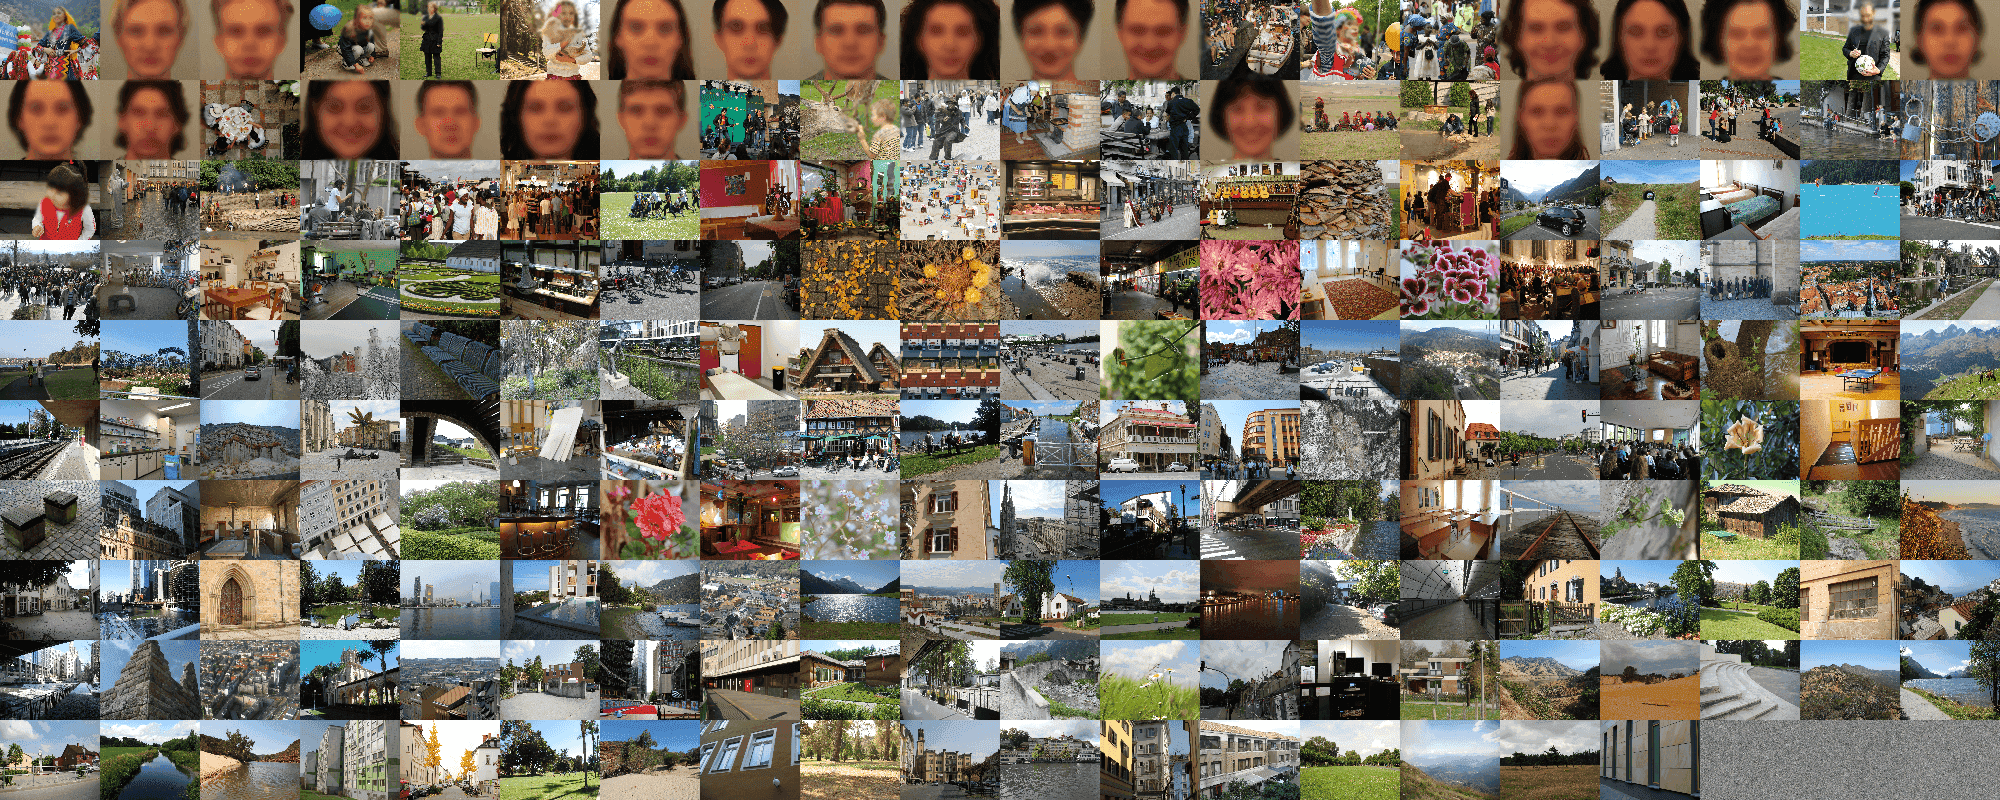
\includegraphics[width = \linewidth]{\imgpath/stimuli_sorted_facesblurred.png}
      \caption{Experimental stimuli, ranked according to the learned global salience. The stimulus with the highest global salience score is on the top-left corner and the rest are sorted with the x-axis changing fastest (row-major order). Faces have been blurred to preserve the identity.}
    \label{fig:globsal-stimuli_sorted}
  \end{subfigure}
  \\
  \begin{subfigure}{\linewidth}
      \centering
      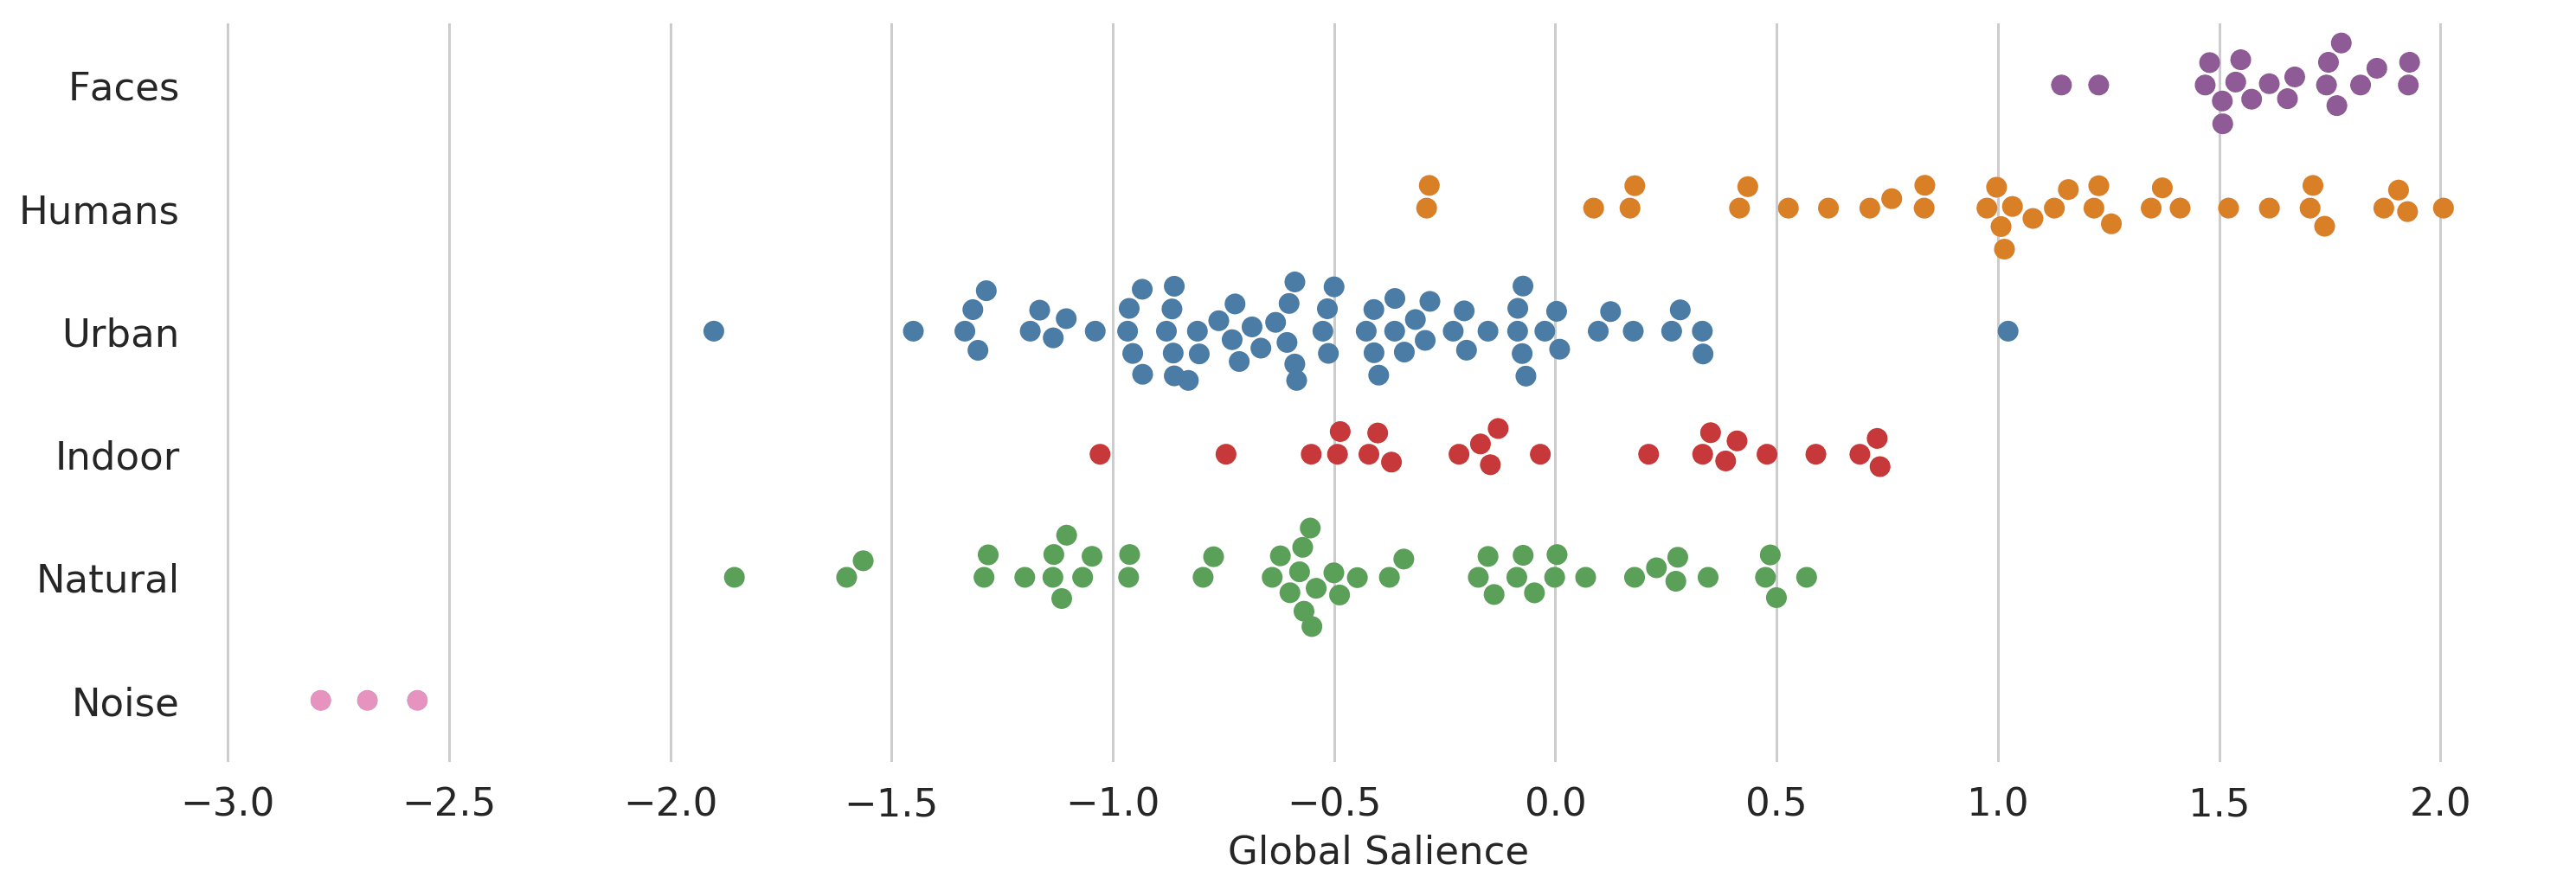
\includegraphics[width = \linewidth]{\imgpath/global_salience.png}
      \caption{Global salience score of each stimulus and image categories.}
    \label{fig:globsal-global_salience_categories}
  \end{subfigure}
  \caption{Global salience scores of the experimental stimuli}
\label{fig:globsal-global_salience}
\end{figure}

Figure~\ref{fig:globsal-global_salience} shows that there exists a clear, general tendency to first fixate on the images that contain either close-up faces or scenes with humans, even though the first fixations may occur, on average, as early as after 242 ms ($\sigma_{SD} = 66$ ms) from the stimulus onset. These two categories, faces and humans, were assigned the highest global salience scores. Then, urban, indoor and natural landscapes obtained significantly lower scores, with no big differences among the three categories. Finally, the three pink-noise images were assigned very low scores, which serves as sanity-check of our proposed method.

\subsection{Global vs. local salience}
\label{sec:results-local_salience}

A reasonable question in view of the results presented in Figure~\ref{fig:globsal-global_salience} is whether the global salience scores---and the ranking of the stimuli that arises from the scores---is a unique measure that assesses the initial visual behaviour when facing competing stimuli, or whether this behaviour and thus our proposed global salience can be explained by the low-level properties of the respective stimuli.

In our second hypothesis (H2) we stated, instead, that the global salience is independent from the low-level local salience properties. So as to test this, we performed several tests, described in Section~\ref{sec:locsal}.

In Figure~\ref{fig:globsal-kld_distr_gbvs} we plot the distribution of the Kullback-Leibler Divergence between the first fixations maps and the GBVS local salience maps of the individual images (see Equation~\ref{eq:kld}). The mean of the distribution is significantly non-zero (two-tail t-test p-value $< .001$, $\mu_{KLD} = 1.44$, $\sigma_{KLD} = 0.33$), which means that there is a significant loss of information when using a local salience map to predict the landing locations of the first fixations on a given image \citep{riche2013saliency}. In order to illustrate the mismatch, in Figure~\ref{fig:globsal-kld_distr_gbvs} we display three example images with the overlaid salience maps and the location of all the first fixations that landed on them. When the KLD value is minimum (a), the salience maps can approximate the fixations, although this happened rarely. Already with KLD values around the mean, the performance of a salience map in predicting the landing location of fixations is rather mediocre (b) and deteriorates further as the KLD increases (c).

\begin{figure}[ht]
  \centering
  \begin{subfigure}{0.75 \linewidth}
      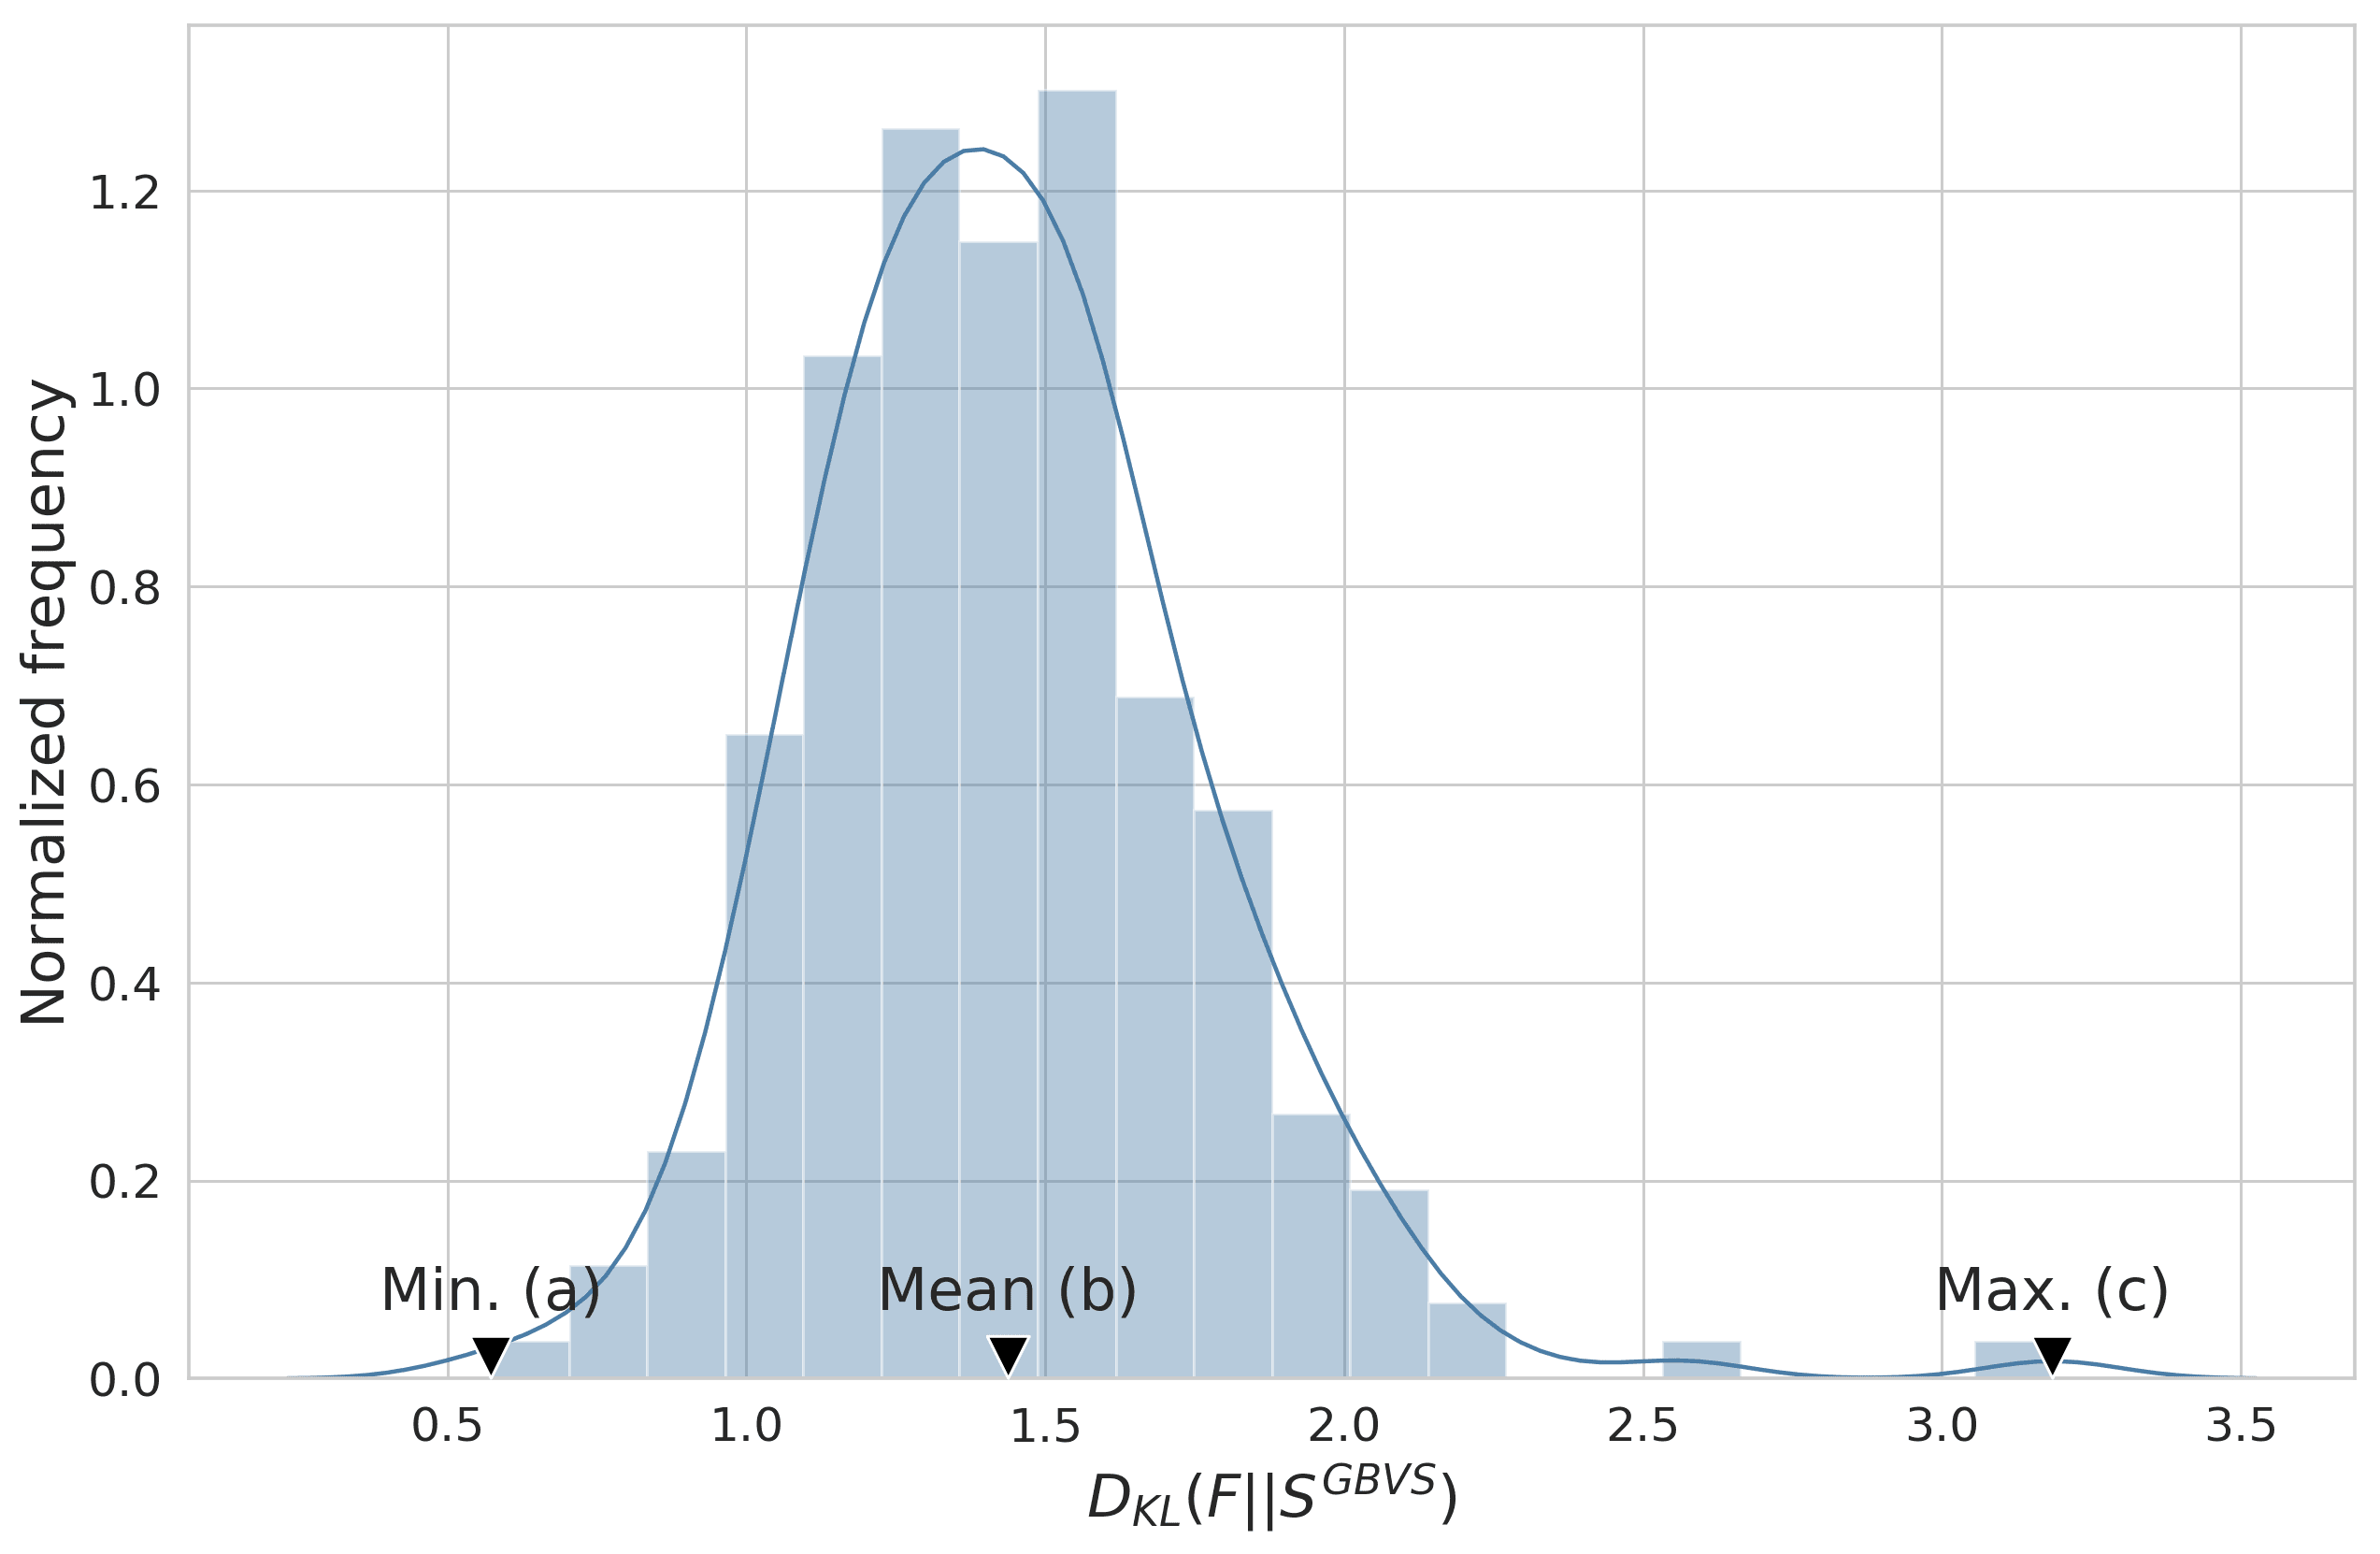
\includegraphics[width = \linewidth]{\imgpath/kld_distr_gbvs.png}
      \label{fig:globsal-kld_distr_gbvs_sub}
  \end{subfigure}
  \\
  \begin{subfigure}{0.3 \linewidth}
      \centering
      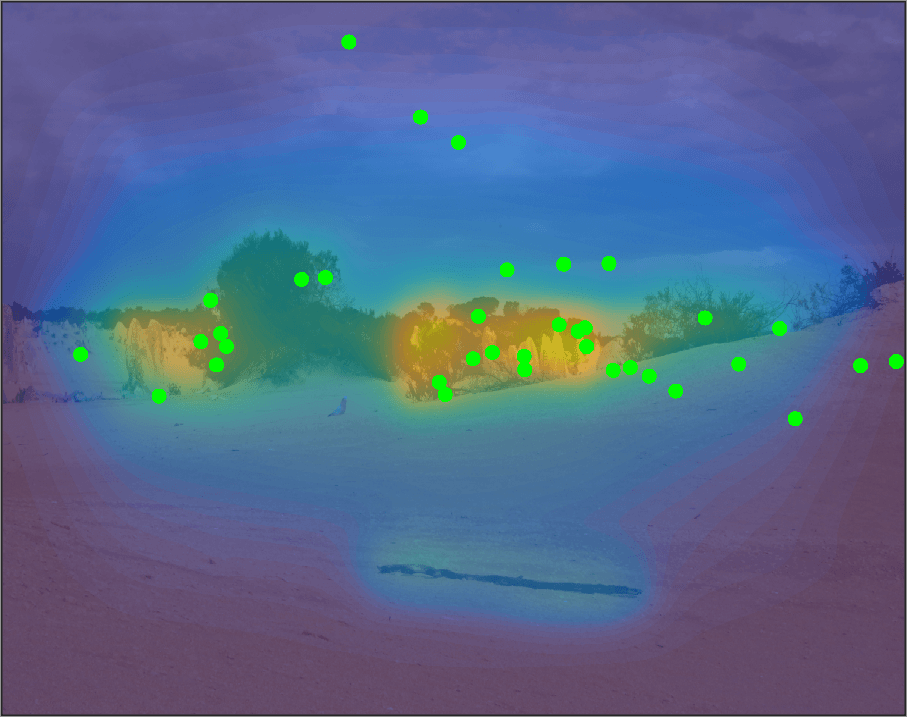
\includegraphics[width = \linewidth]{\imgpath/kld_gbvs_min_image.png}
      \caption{$D_{KL}(F||S) = 0.57$}
    \label{fig:globsal-kld_gbvs_min_image}
  \end{subfigure}
  \hspace{0.02 \linewidth}
  \begin{subfigure}{0.3 \linewidth}
      \centering
      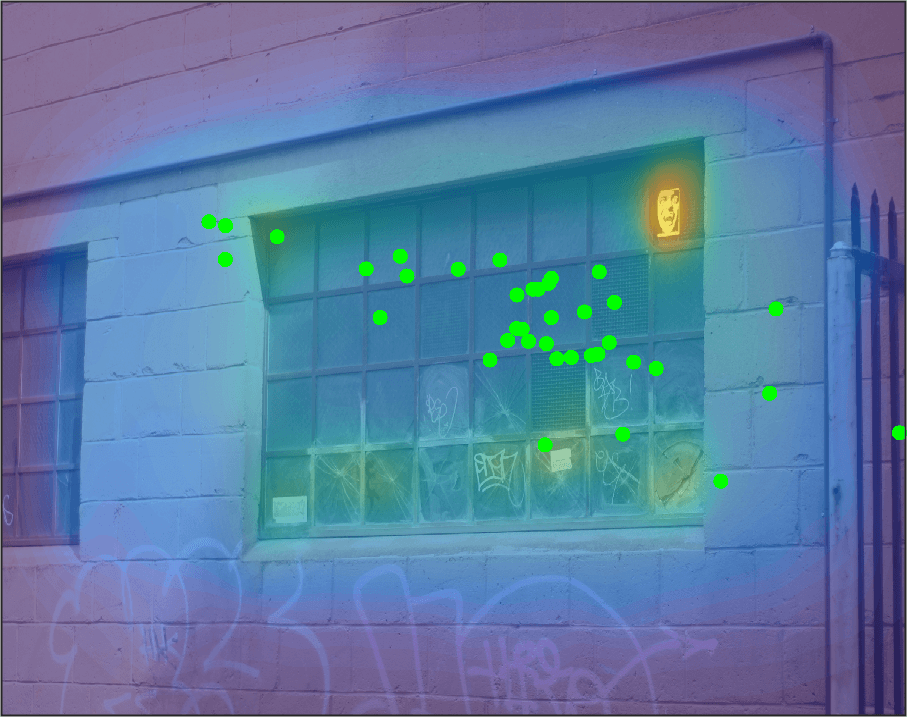
\includegraphics[width = \linewidth]{\imgpath/kld_gbvs_mean_image.png}
      \caption{$D_{KL}(F||S) = 1.44$}
    \label{fig:globsal-kld_gbvs_mean_image}
  \end{subfigure}
  \hspace{0.02 \linewidth}
  \begin{subfigure}{0.3 \linewidth}
      \centering
      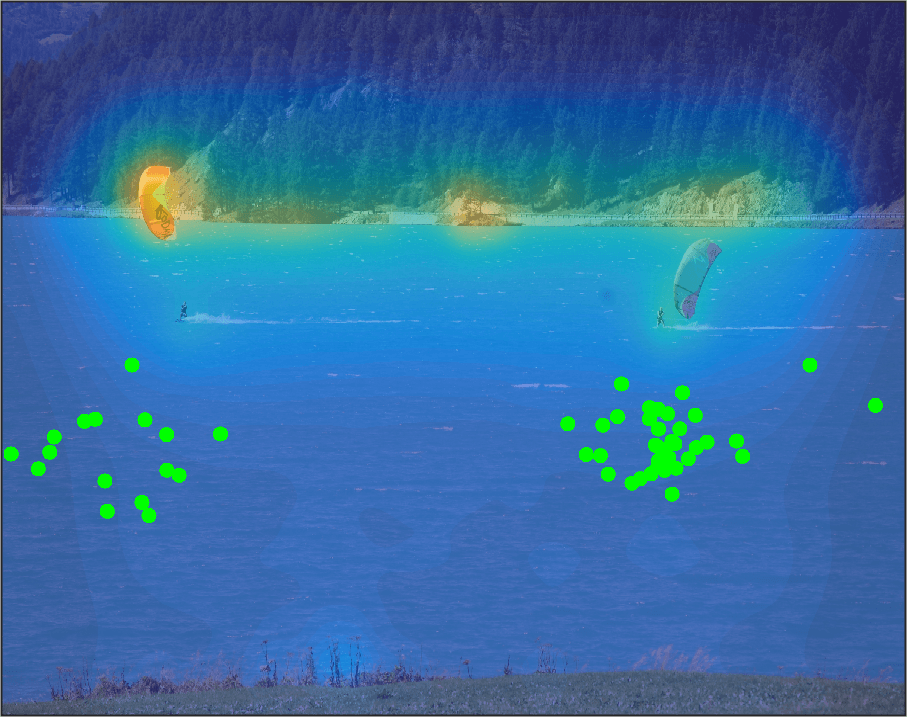
\includegraphics[width = \linewidth]{\imgpath/kld_gbvs_max_image.png}
      \caption{$D_{KL}(F||S) = 3.19$}
    \label{fig:globsal-kld_gbvs_max_image}
  \end{subfigure}
  \caption{Top row: distribution of the Kullback-Leibler Divergence between the first fixations map and the GBVS local salience maps. Bottom row: images with the minimum, closest to the mean and maximum KLD, with their overlaid salience map and the location of the first fixations.}
\label{fig:globsal-kld_distr_gbvs}
\end{figure}

Perhaps not surprisingly, in view of the poor match between the salience maps and the first fixation maps, Figure~\ref{fig:globsal-kld_vs_globsal_gbvs} shows that the Kullback-Leibler Divergence between them does not correlate with the global salience scores. This means that the images which attract the first fixations towards salient regions (low KLD) do not tend to have high global salience scores neither vice versa.

\begin{figure}[ht]
  \centering
  \begin{subfigure}{0.6 \linewidth}
      
\includegraphics[width = \linewidth]{\imgpath/legend_categories.png}
  \end{subfigure}
  \\
  \begin{subfigure}{0.48 \linewidth}
      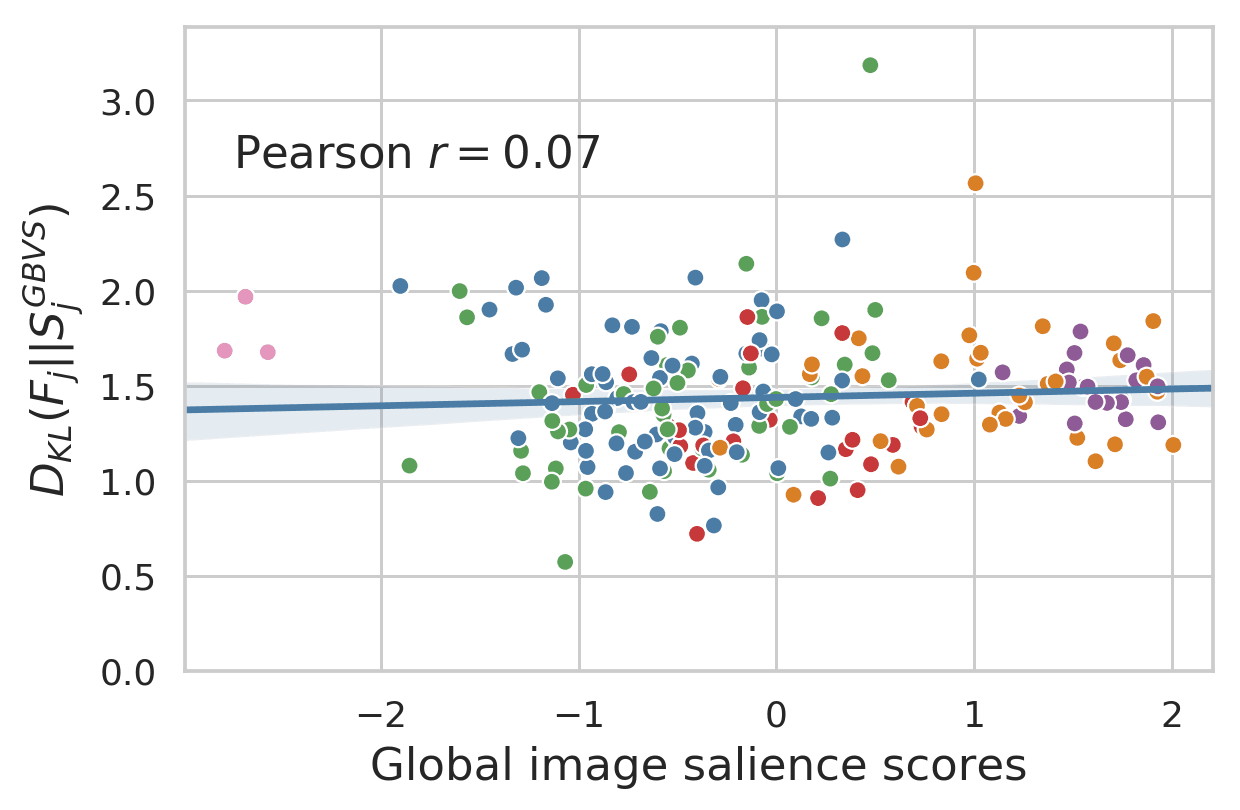
\includegraphics[width = \linewidth]{\imgpath/kld_vs_globsal_gbvs.png}
      \caption{GBVS}
    \label{fig:globsal-kld_vs_globsal_gbvs}
  \end{subfigure}
  \hspace{0.01 \linewidth}
  \begin{subfigure}{0.48 \linewidth}
      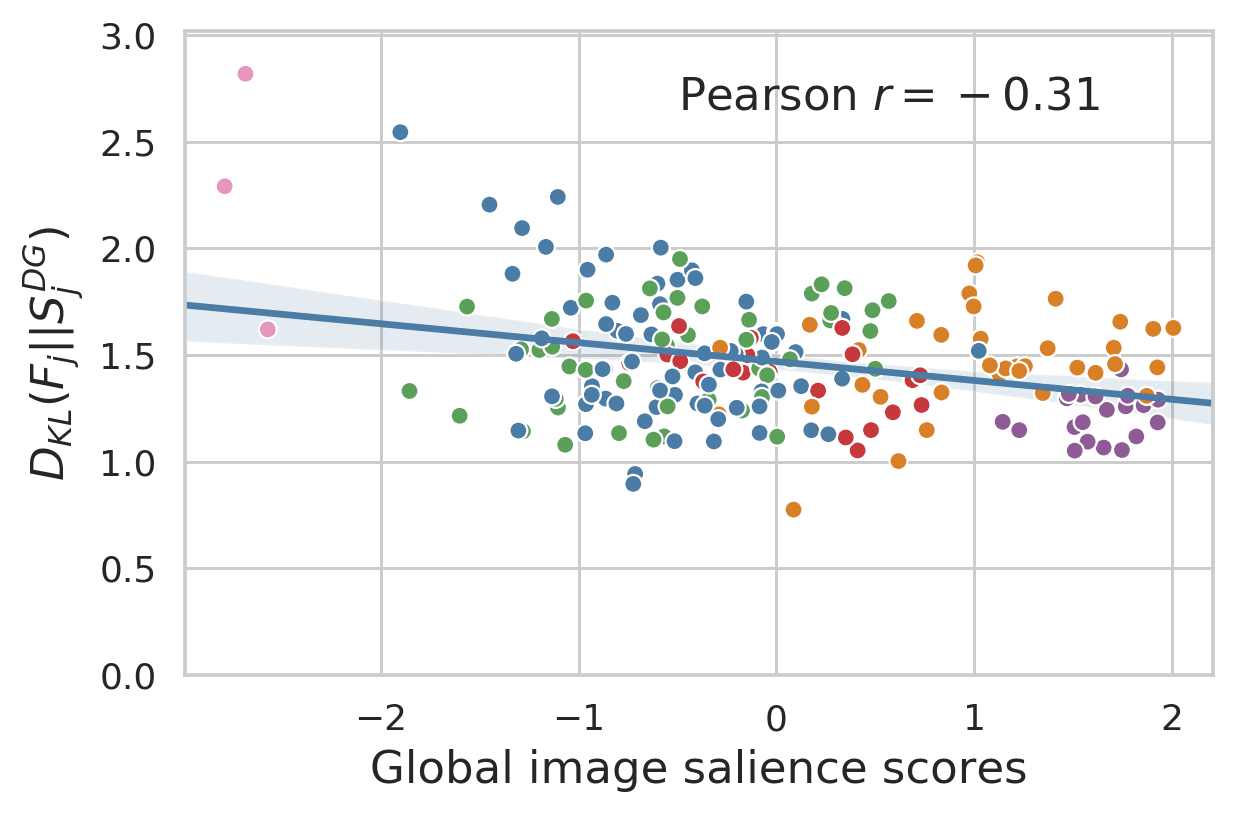
\includegraphics[width = \linewidth]{\imgpath/kld_vs_globsal_deepgaze.png}
      \caption{Deep Gaze}
    \label{fig:globsal-kld_vs_globsal_deepgaze}
  \end{subfigure}
  \caption{Comparison between the global salience scores the KLD between the first fixation distribution and the salience maps from the computational models}
  \label{fig:globsal-kld_vs_globsal}
\end{figure}

Finally, we analyse in Figure~\ref{fig:globsal-mass_gbvs_vs_globsal} whether the direction of the first fixation when looking at competing stimuli, as modelled by our proposed global salience scores, can be explained by the difference in the low-level salience properties of the competing stimuli, as measured by the GBVS salience mass of each image (see Section~\ref{sec:locsal-glob_vs_loc}). Also in this case we found no significant correlation.

The noisy images included in the stimulus set serve once more as a validation of the expected results. When one of the images (left or right) was pink noise the difference in GBVS salience mass was either very high or very low, as is the difference in global salience scores. In this case, both metrics do correlate, but as shown by the central scatter plot of Figure~\ref{fig:globsal-mass_gbvs_vs_globsal}, the feature-driven (GBVS) salience mass cannot explain the global salience scores learned by the model.

\begin{figure}[ht]
  \centering
  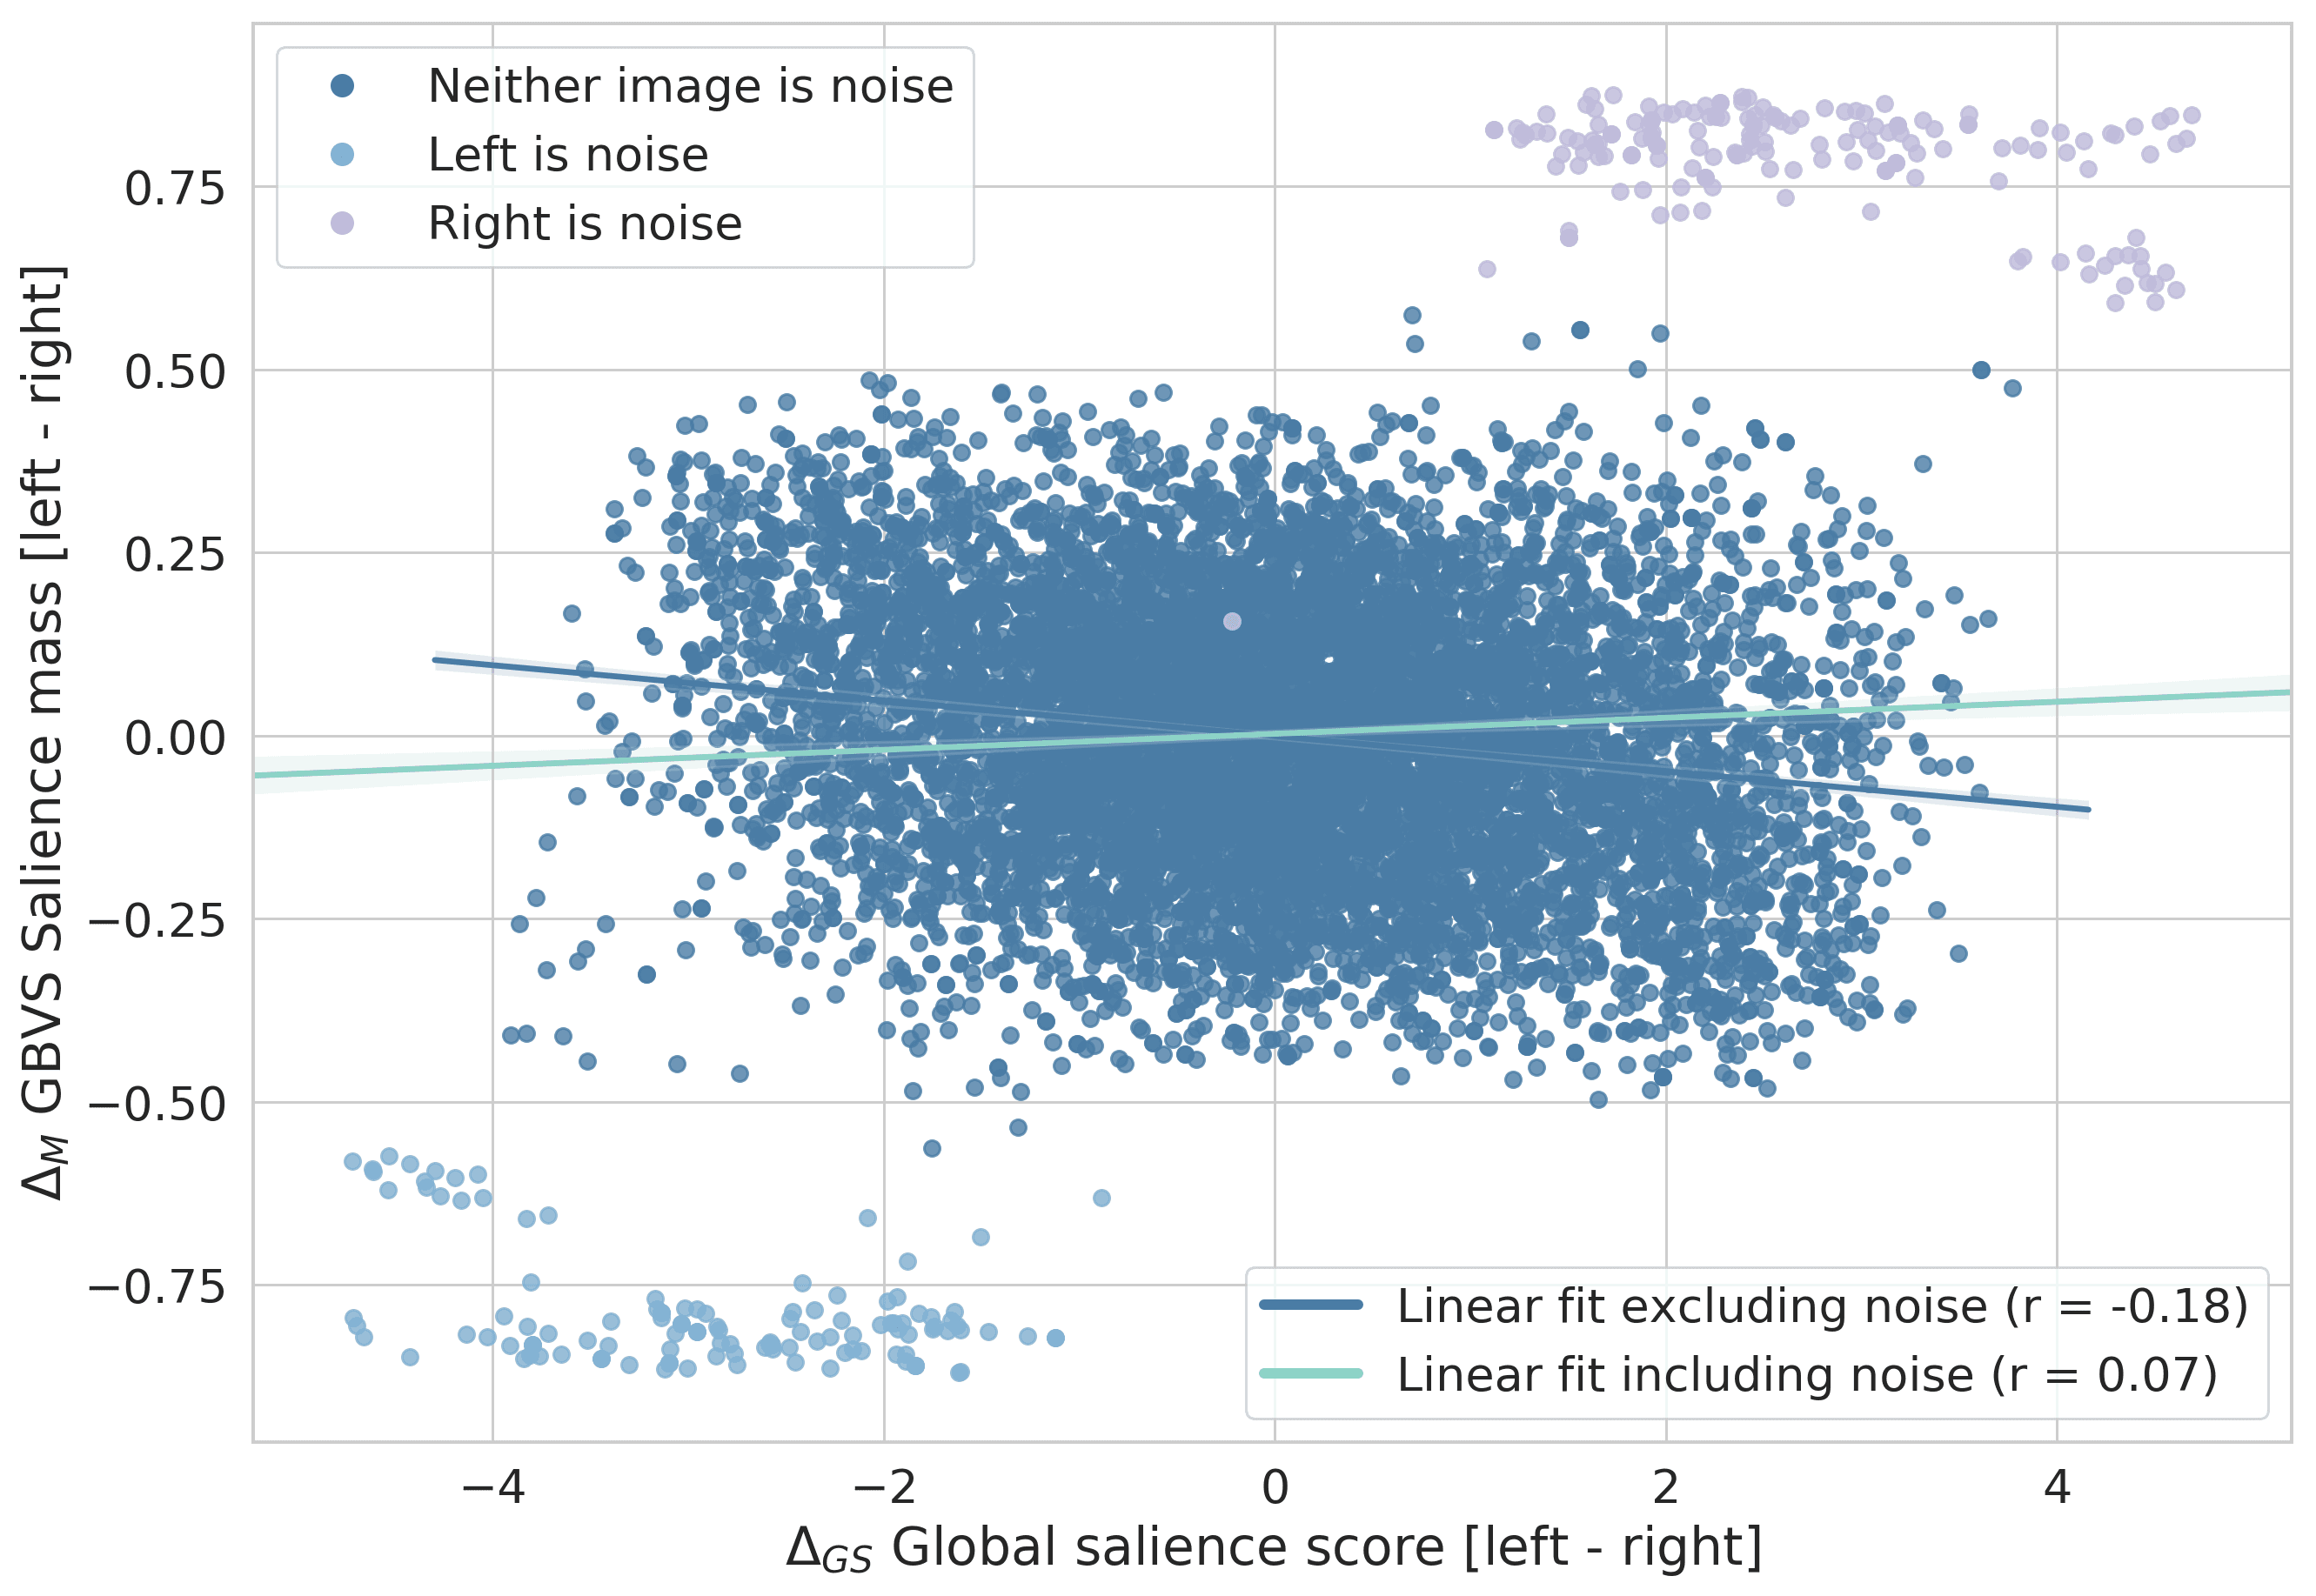
\includegraphics[width = \linewidth]{\imgpath/mass_gbvs_vs_globsal.png}
  \caption{Correlation between the GBVS image salience mass and the global salience scores.}
\label{fig:globsal-mass_gbvs_vs_globsal}
\end{figure}

In order to better understand what drives the direction of the first fixation when faced with competing stimuli, we also compared our proposed global salience with properties of Deep Gaze II salience maps. As presented in Section~\ref{sec:locsal}, unlike GBVS, Deep Gaze does make use of higher-level information of the images to predict the salience maps, since it is a neural network pre-trained on image object recognition tasks. This allows it to model salience driven by faces or objects \citep{kuemmerer2017icfdeepgaze} and it becomes an interesting model to which compare our global salience model, since we have seen in Section~\ref{sec:results-global_salience} that images containing faces and humans tend to get a higher global salience score.

In general, we observe that unlike GBVS, measures derived from Deep Gaze salience maps exhibit a non-zero, yet moderate correlation with our proposed global salience. For instance, Figure~\ref{fig:globsal-kld_vs_globsal_deepgaze} shows a slight negative correlation between global salience scores and the KLD between first fixation distributions and Deep Gaze salience maps. However, looking at the distribution of the Kullback-Leibler divergence in Figure~\ref{fig:globsal-kld_distr_deepgaze}, we see that the salience maps are also far from matching the location of the first fixations on the images. Finally, we also observed (see Figure~\ref{fig:globsal-mass_deepgaze_vs_globsal} a non-zero correlation between the difference of global salience scores between the left and the right image, and the difference in salience mass computed with Deep Gaze.

\begin{figure}[ht]
  \centering
  \begin{subfigure}{0.75 \linewidth}
      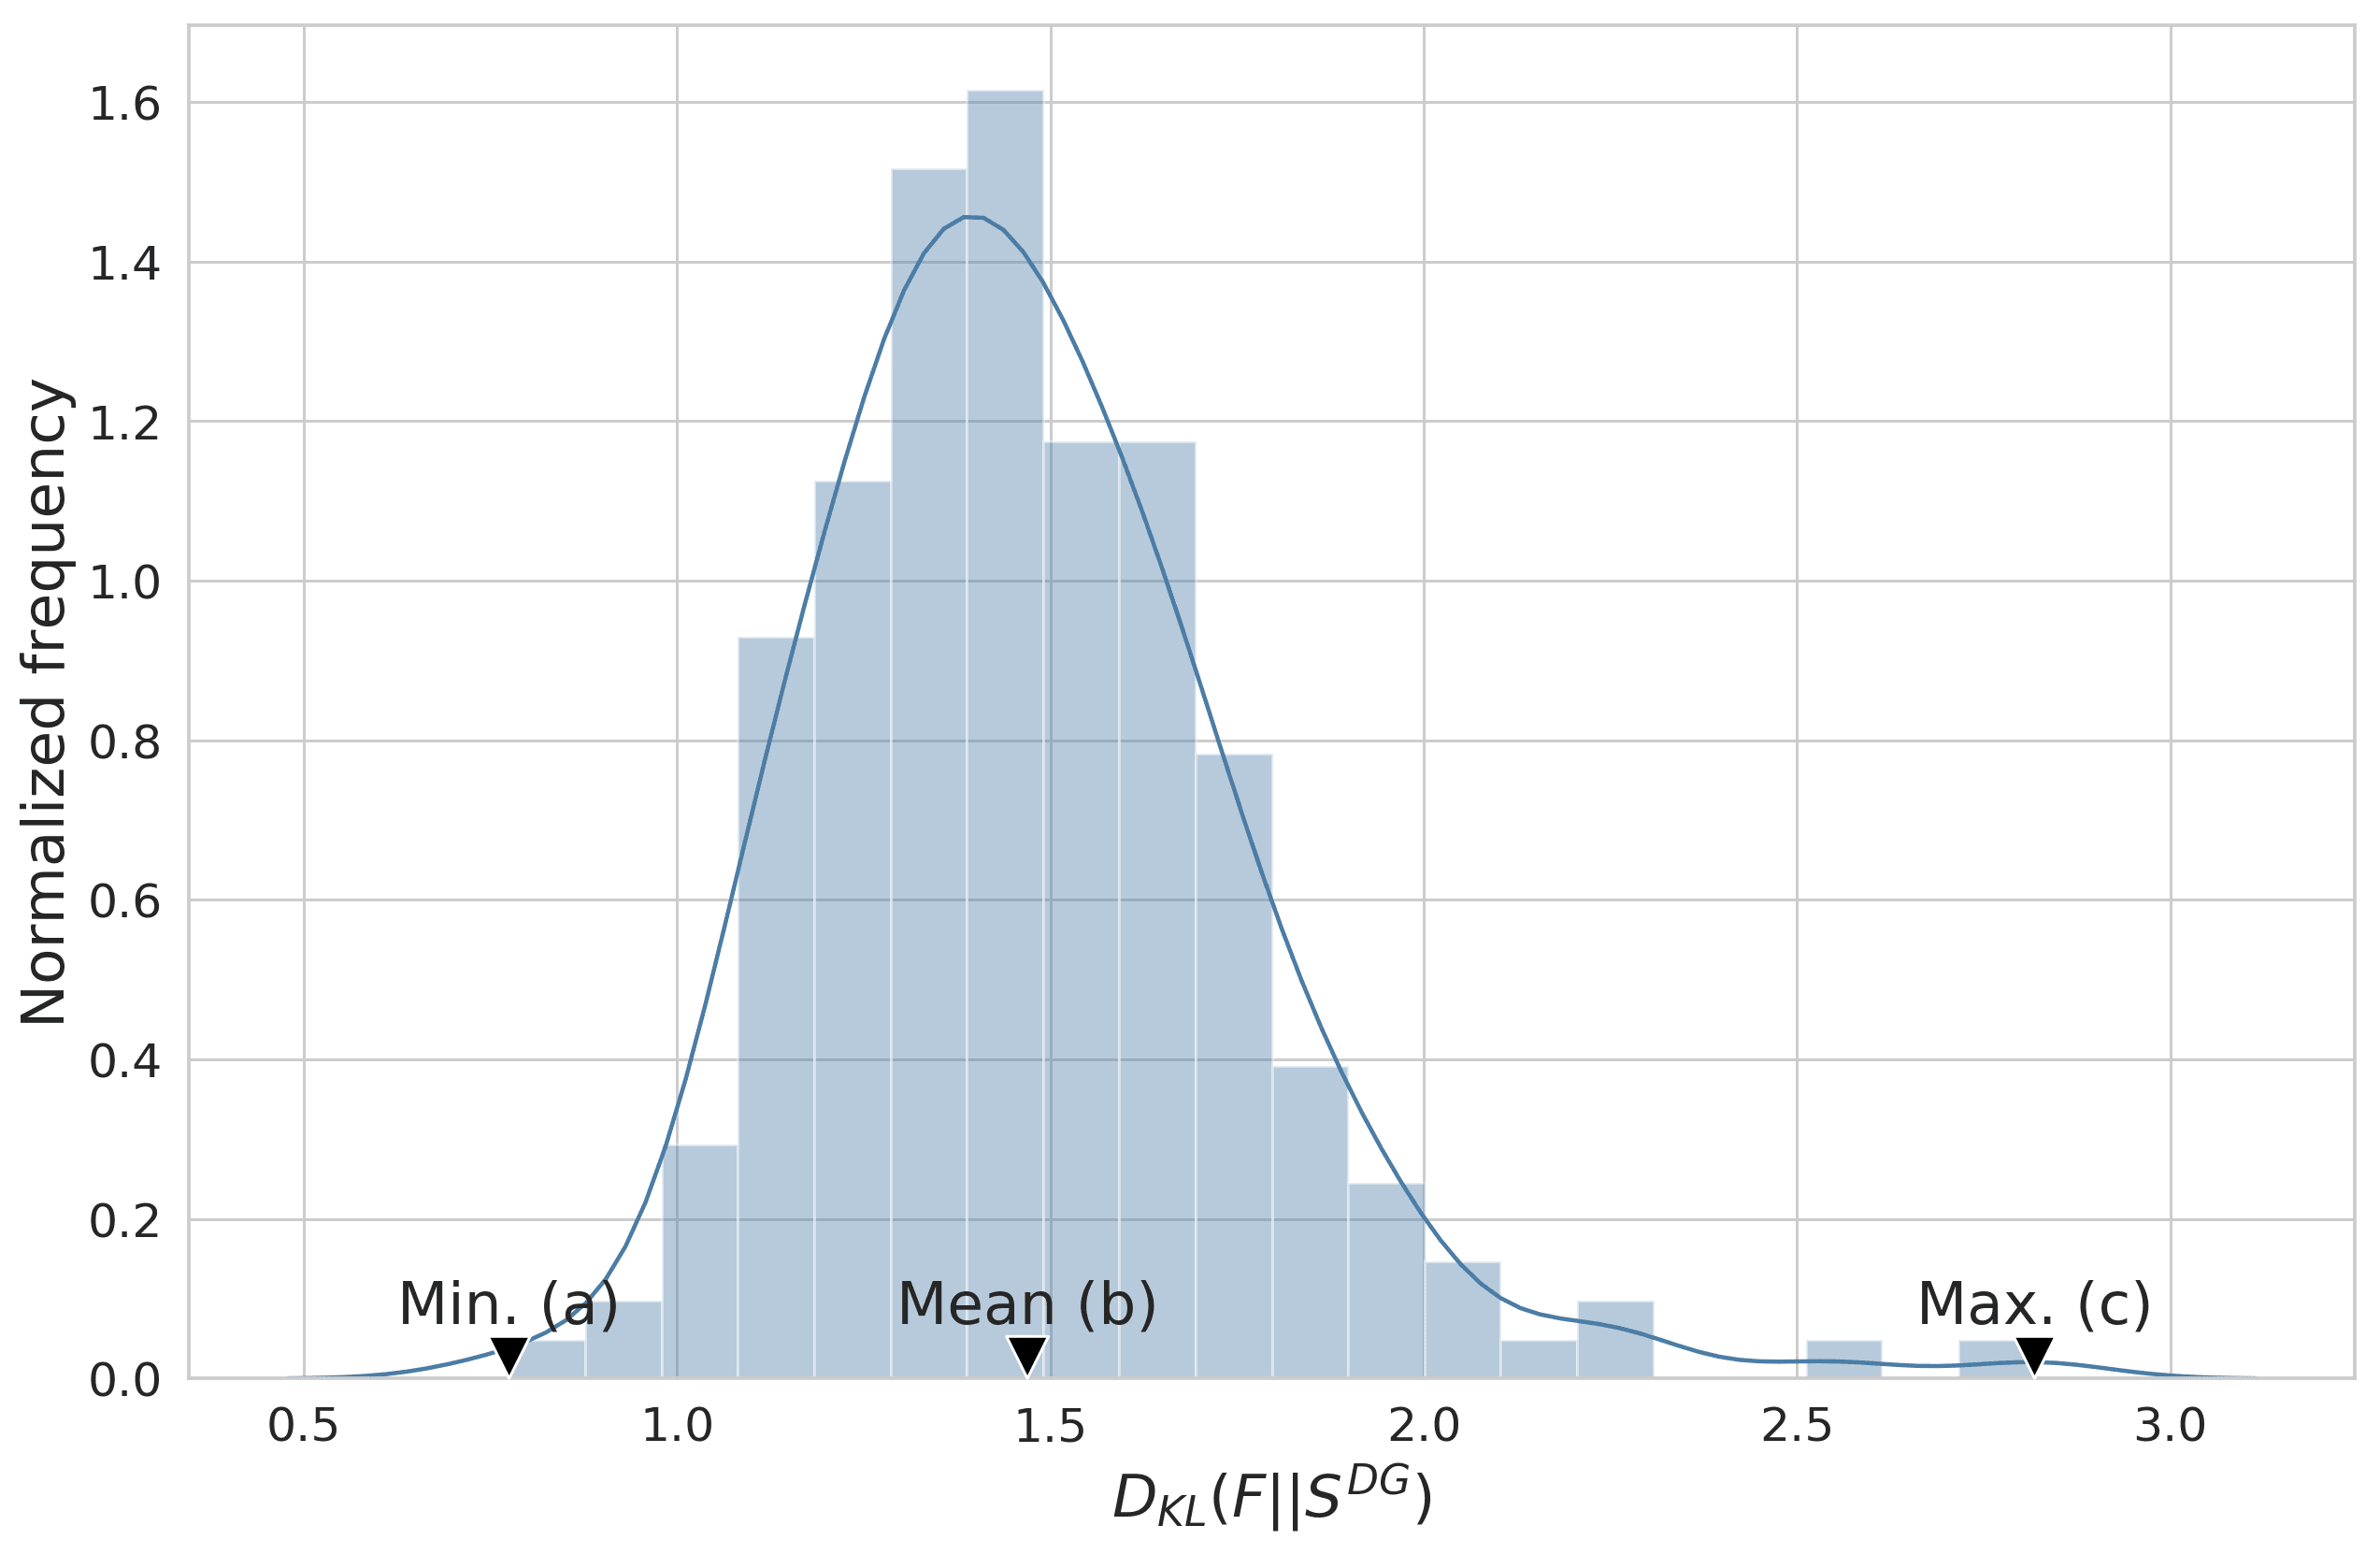
\includegraphics[width = \linewidth]{\imgpath/kld_distr_deepgaze.png}
      \label{fig:globsal-kld_distr_deepgaze_sub}
  \end{subfigure}
  \\
  \begin{subfigure}{0.3 \linewidth}
      \centering
      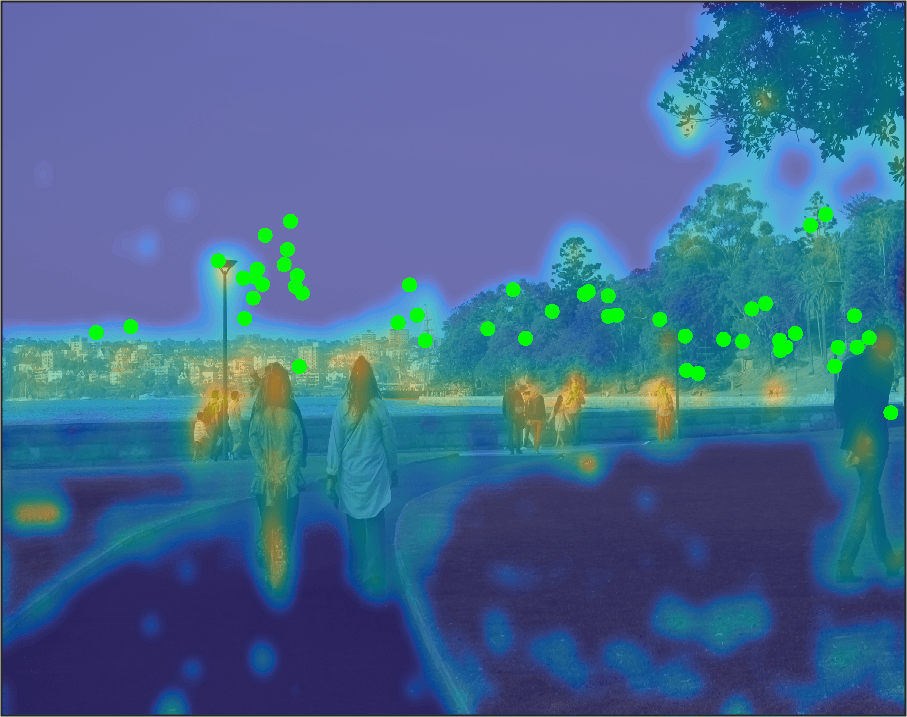
\includegraphics[width = \linewidth]{\imgpath/kld_deepgaze_min_image.png}
      \caption{$D_{KL}(F||S) = 0.57$}
    \label{fig:globsal-kld_deepgaze_min_image}
  \end{subfigure}
  \hspace{0.02 \linewidth}
  \begin{subfigure}{0.3 \linewidth}
      \centering
      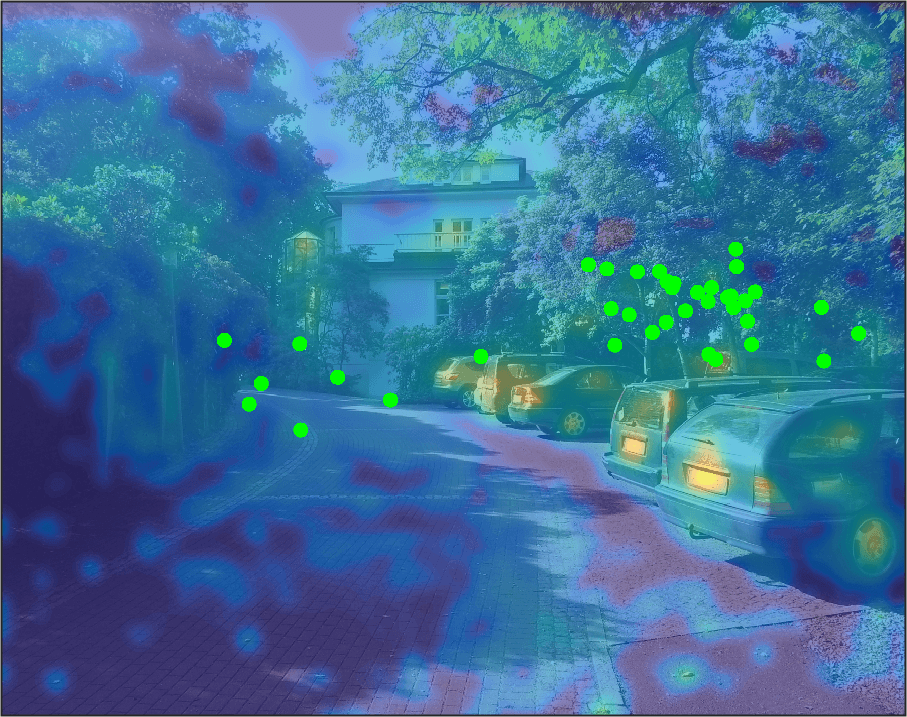
\includegraphics[width = \linewidth]{\imgpath/kld_deepgaze_mean_image.png}
      \caption{$D_{KL}(F||S) = 1.44$}
    \label{fig:globsal-kld_deepgaze_mean_image}
  \end{subfigure}
  \hspace{0.02 \linewidth}
  \begin{subfigure}{0.3 \linewidth}
      \centering
      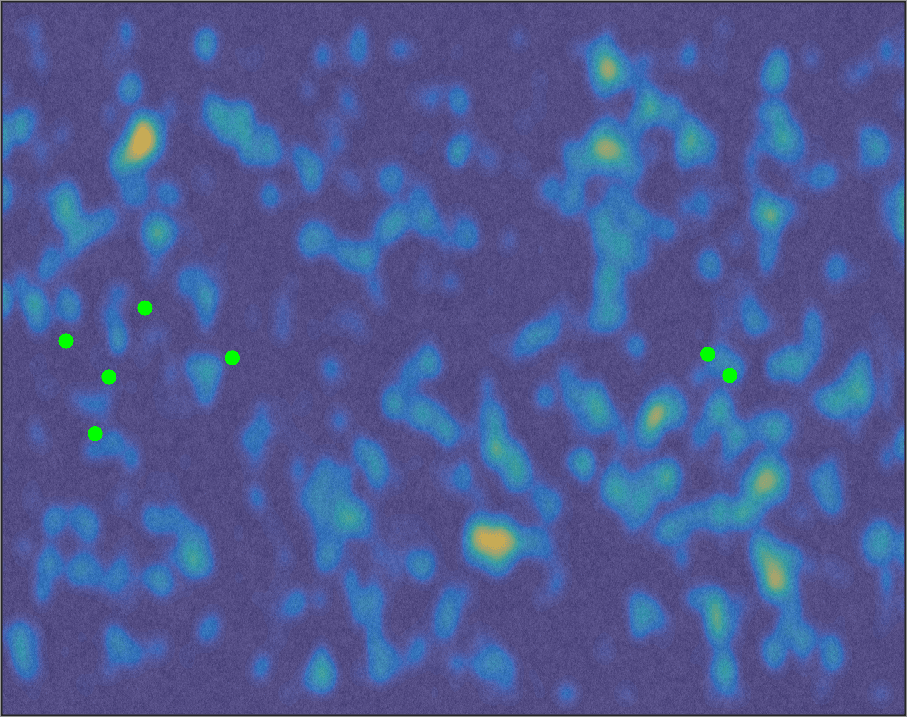
\includegraphics[width = \linewidth]{\imgpath/kld_deepgaze_max_image.png}
      \caption{$D_{KL}(F||S) = 3.19$}
    \label{fig:globsal-kld_deepgaze_max_image}
  \end{subfigure}
  \caption{Top row: distribution of the Kullback-Leibler Divergence between the first fixations map and the Deep Gaze local salience maps. Bottom row: images with the minimum, closest to the mean and maximum KLD, with their overlaid salience map and the location of the first fixations.}
  \label{fig:globsal-kld_distr_deepgaze}
\end{figure}

\begin{figure}[ht]
  \centering
  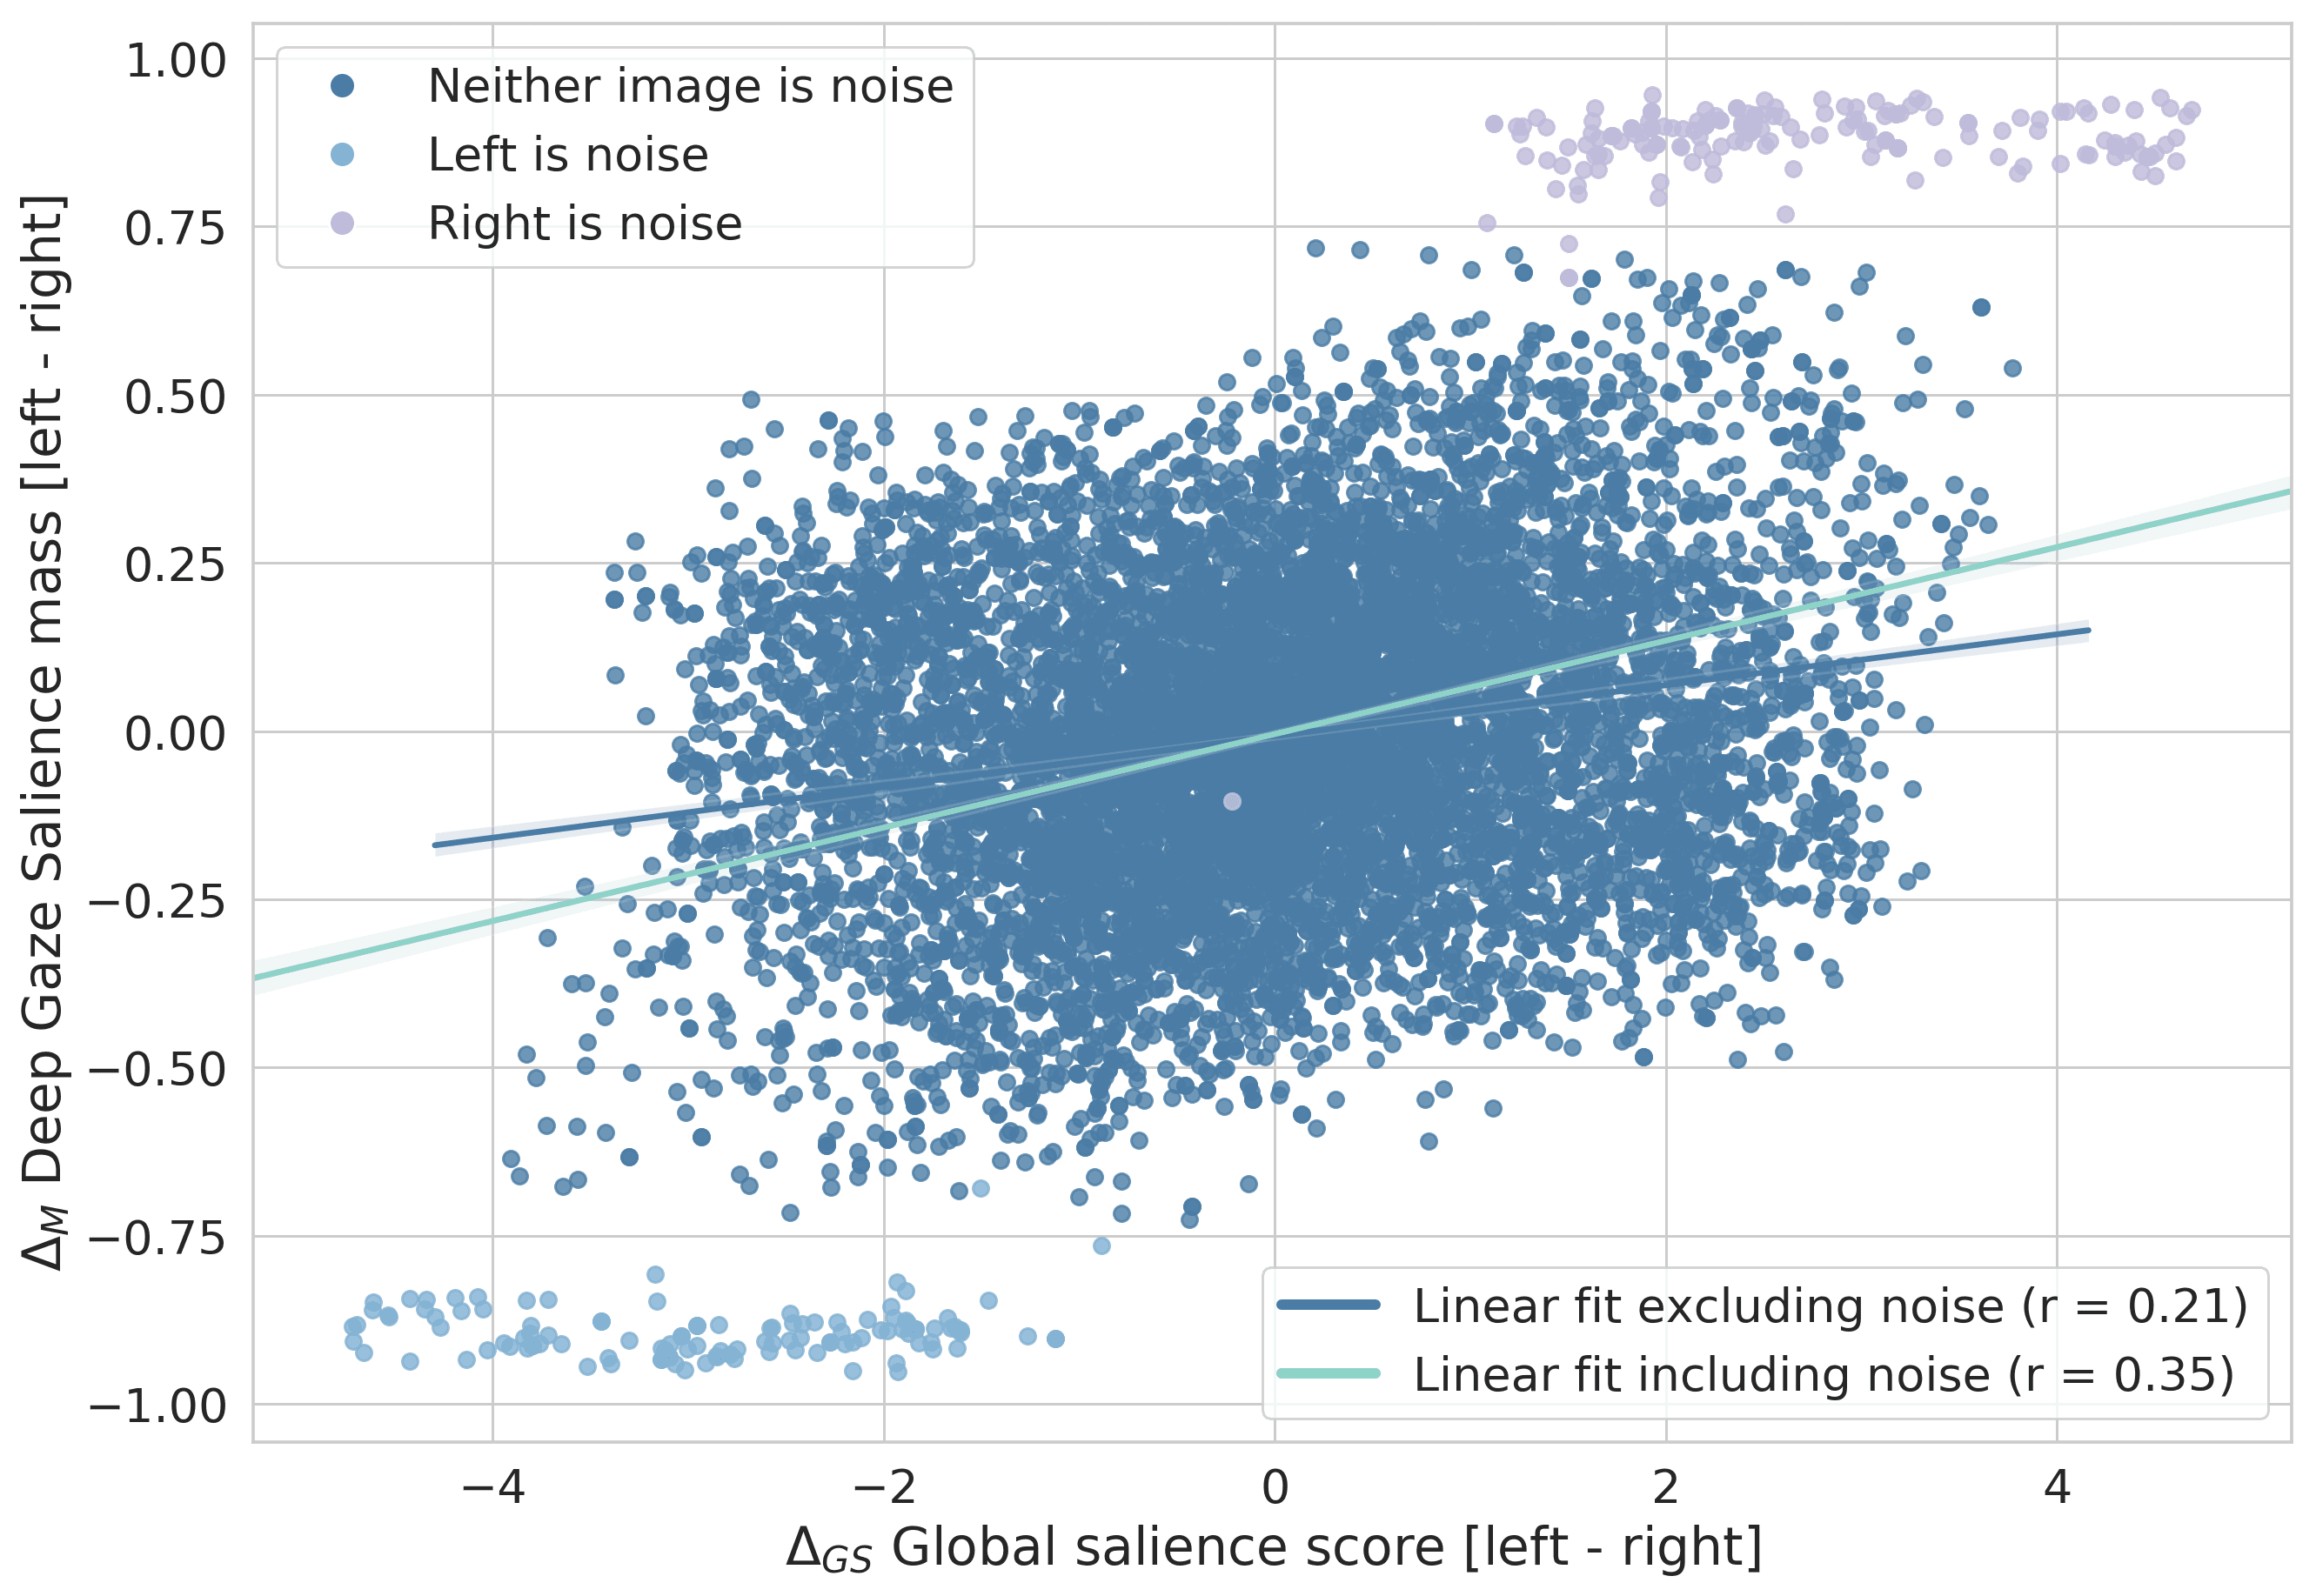
\includegraphics[width = \linewidth]{\imgpath/mass_deepgaze_vs_globsal.png}
  \caption{Correlation between the Deep Gaze image salience mass and the global salience scores.}
\label{fig:globsal-mass_deepgaze_vs_globsal}
\end{figure}

Taken together, we can conclude that our proposed computational model provided a robust method to rank images according to a unique global image salience that is independent of the low-level local salience properties of the stimuli, and we observed a non-zero, yet moderate correlation with a computational salience model that incorporates higher-level cues.

\subsection{Lateral bias}
\label{sec:results-spatialbias}
Our third hypothesis (H3) stated that a general spatial bias leads to a higher likelihood to first fixate on the left rather than the right image. We thus calculated the number of first saccades that landed onto the left and the right image for each block separately (Figure~\ref{fig:globsal-first_saccade_blocks}). A 4 $\times$ 2 (block: 1, 2, 3, 4 $\times$ image side: left, right) repeated measures ANOVA (Greenhouse-Geisser corrected) revealed a general spatial bias of the initial saccade towards the left image as indicated by a significant main effect according to the image side [\textit{F}(1, 48) = 30.833; \textit{p} \textless\ .001; \textit{$\eta_p^2$} = .391]. No further effects were found [all \textit{F} $\leq$ 2.594; all \textit{p} $\geq$.074, all \textit{$\eta_p^2$} $\leq$ .051], showing that the left bias was present in all blocks with similar extent. Thus, we can conclude that the participants generally targeted their initial saccades more on left than right sided images.

\begin{figure}[ht]
  \centering
  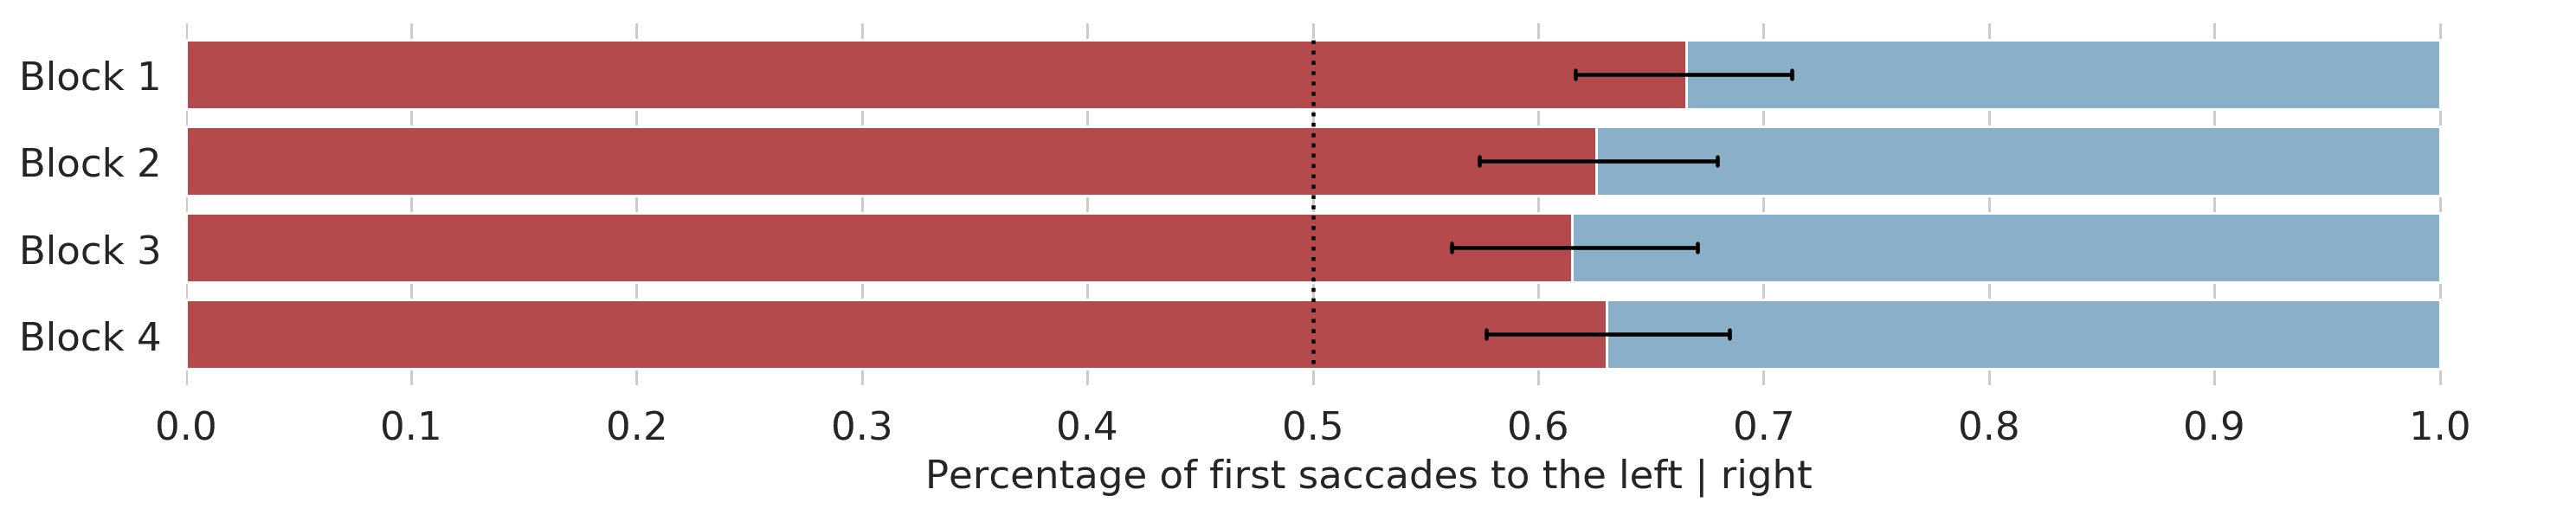
\includegraphics[width = \linewidth]{\imgpath/first_saccade_blocks.png}
  \caption{Percentage of first saccades that targeted on the left (red) and right (blue) images, at each block of the experimental session. Error bars depict the standard deviation of the mean. Note that considerably more first fixations landed on the left image, highlighting the lateral bias.}
\label{fig:globsal-first_saccade_blocks}
\end{figure}

Nonetheless, the error bars in Figure~\ref{fig:globsal-first_saccade_blocks} suggest a high variability of the lateral bias across subjects. In order to investigate this, we calculated the number of first saccades on the right image for each participant separately. Moreover, since our model included an individual bias term for each participant, as described in Section~\ref{sec:globsal}, we can also look at the magnitude of the coefficients learned by the model. In Figure~\ref{fig:globsal-subject_bias} we plot, for each participant, the percentage of first saccades towards the right image and their corresponding lateral bias term learned by the computational model. Both metrics are highly correlated---further highlighting the validity of the model---and reveal a high variability in the lateral bias across participants. Overall, 63 \% of all first fixations landed on the left image.

\begin{figure}[ht]
  \centering
  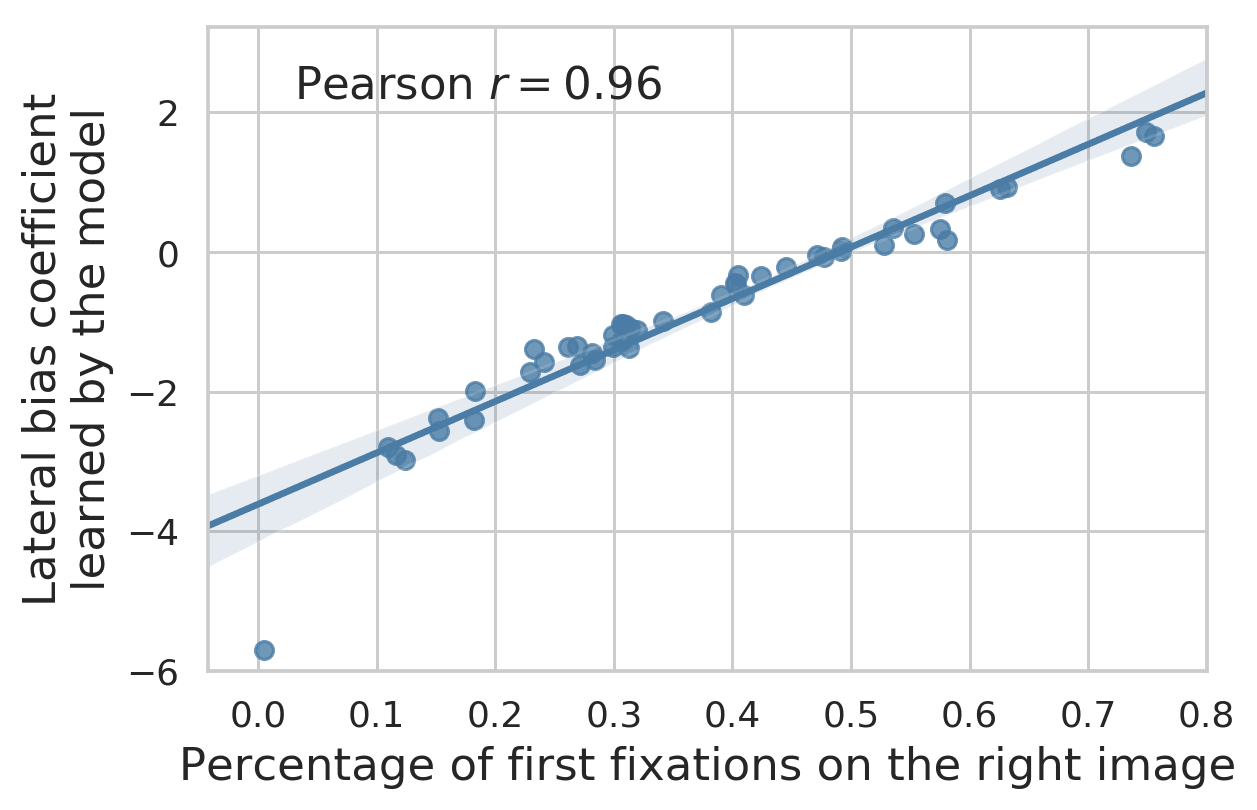
\includegraphics[width = 0.6 \linewidth]{\imgpath/subject_bias.png}
  \caption{Lateral bias of each participant, as measured by the percentage of first fixations onto the right image and the lateral bias terms learned by our computational model. Both metrics are highly correlated and reveal the average left bias, but with high variability across participants.}
\label{fig:globsal-subject_bias}
\end{figure}

\subsection{Task and familiarity}
\label{sec:results-taskandfam}
Next, we investigated the effect of the familiarity with one of the images and of the task of selecting the already seen or unseen image, which the participants had to perform in blocks 2 and 3 of the experiment, respectively. In particular, we were interested in finding out whether there is a tendency to direct the initial saccade towards the task-relevant images or towards the new images, for instance. In our fourth hypothesis (H4) we stated that our task and familiarity should have little or no influence in the initial saccade. For that purpose, we first performed a 2 $\times$ 2 (task: select new, select old $\times$ fixated image: new image, old image) repeated measures ANOVA analysis (Greenhouse-Geisser corrected). The results revealed no significant effects [all \textit{F} $\leq$ 1.936; all \textit{p} $\geq$ .170, all \textit{$\eta_p^2$} $\leq$ .039] (Figure~\ref{fig:globsal-first_saccade_tasks}). Thus, the provided tasks did not bias the initial saccade decision to target one of the two presented images. Nevertheless, we found that participants correctly identified 91.43\% of the new images in block 2 and 91.16\% of the old images in block 3. Hence, the task performance was highly above chance (50\%) and the participants were accurate in identifying the new and old images respectively.

Also in this case, the same conclusion can be extracted from the coefficients learned by the model to capture the task and familiarity effects, which are -0.04 and -0.10, respectively, that is, very small and only slightly higher for the familiarity.

\begin{figure}[ht]
  \centering
  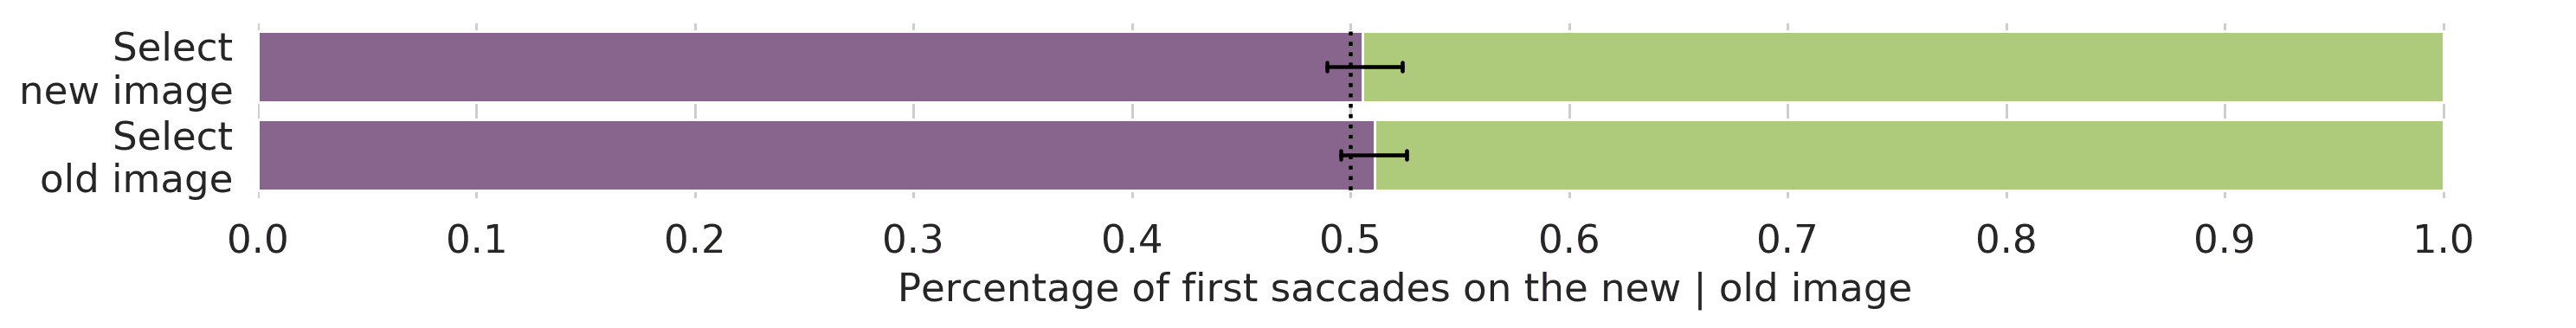
\includegraphics[width = \linewidth]{\imgpath/first_saccade_tasks.png}
  \caption{Percentage of first saccades that targeted on the new (purple) and old (green) images, at blocks 2 and 3, where participants had the task of indicating the new and old image, respectively. Error bars depict the standard deviation of the mean. No significant bias can be appreciated in this case.}
\label{fig:globsal-first_saccade_tasks}
\end{figure}

Taken together, spatial properties influenced the initial saccade in favour to fixate left sided images first. Although task performance was very high, neither the task nor the familiarity with one of the images had an influence in the direction of the first fixation after stimulus onset. These results fully support our third and fourth hypotheses.

\subsection{Total exploration of images}
\label{sec:results-totalexplorationofimages}
In our fifth hypothesis (H5), we stated that images with higher global image salience lead to a longer exploration time than images with lower global salience. We thus calculated the relative dwell time on each image, left and right, for each trial. As an initial step, similarly to the analysis of the initial saccade, we analysed the potential effect of the spatial image location as well as the task and familiarity relevance on the exploration time. 

With respect to the spatial image location, a 4 $\times$ 2 (block: 1, 2, 3, 4 $\times$ image side: left, right) repeated measures ANOVA (Greenhouse-Geisser corrected) revealed a significant main effect according to the block [\textit{F}(2.368, 113.668) = 12.066; \textit{p} \textless\ .001; \textit{$\eta_p^2$} = .201] but no further effects [all \textit{F} $\leq$ 2.232; all \textit{p} $\geq$.109, all \textit{$\eta_p^2$} $\leq$ .044]. Thus, the total time of exploration did not depend on the spatial location of the images, as also shown in Figure \ref{fig:globsal-dwell_blocks}. 

With respect to the task relevance---recall: block 2 - select new image; block 3 - select old image---we calculated a 2 $\times$ 2---task: select new, select old $\times$ fixated image: new image, old image---repeated measures ANOVA (Greenhouse-Geisser corrected). The results revealed a significant main effect according to the task [\textit{F}(1, 48) = 4.298; \textit{p} \textless\ .050; \textit{$\eta_p^2$} = .082] and fixated image [\textit{F}(1, 48) = 64.524; \textit{p} \textless\ .001; \textit{$\eta_p^2$} = .573], as well as an interaction between task and fixated image [\textit{F}(1, 48) = 36.728; \textit{p} \textless\ .001; \textit{$\eta_p^2$} = .433]. As shown by Figure \ref{fig:globsal-dwell_fam_task}, our results showed that, in general, participants tended to spend more time exploring new instead of previously seen images. Furthermore, this effect was noticeably larger in block 2, where the task was to select the new images, than in block 3 (select old image). 

Consequently, we found that the spatial location of images did not affect the total time of exploration. Instead, the task and familiarity had a considerable impact on the exploration time, revealing that new images were explored during a longer time than the counterpart.

\begin{figure}[ht]
  \centering
  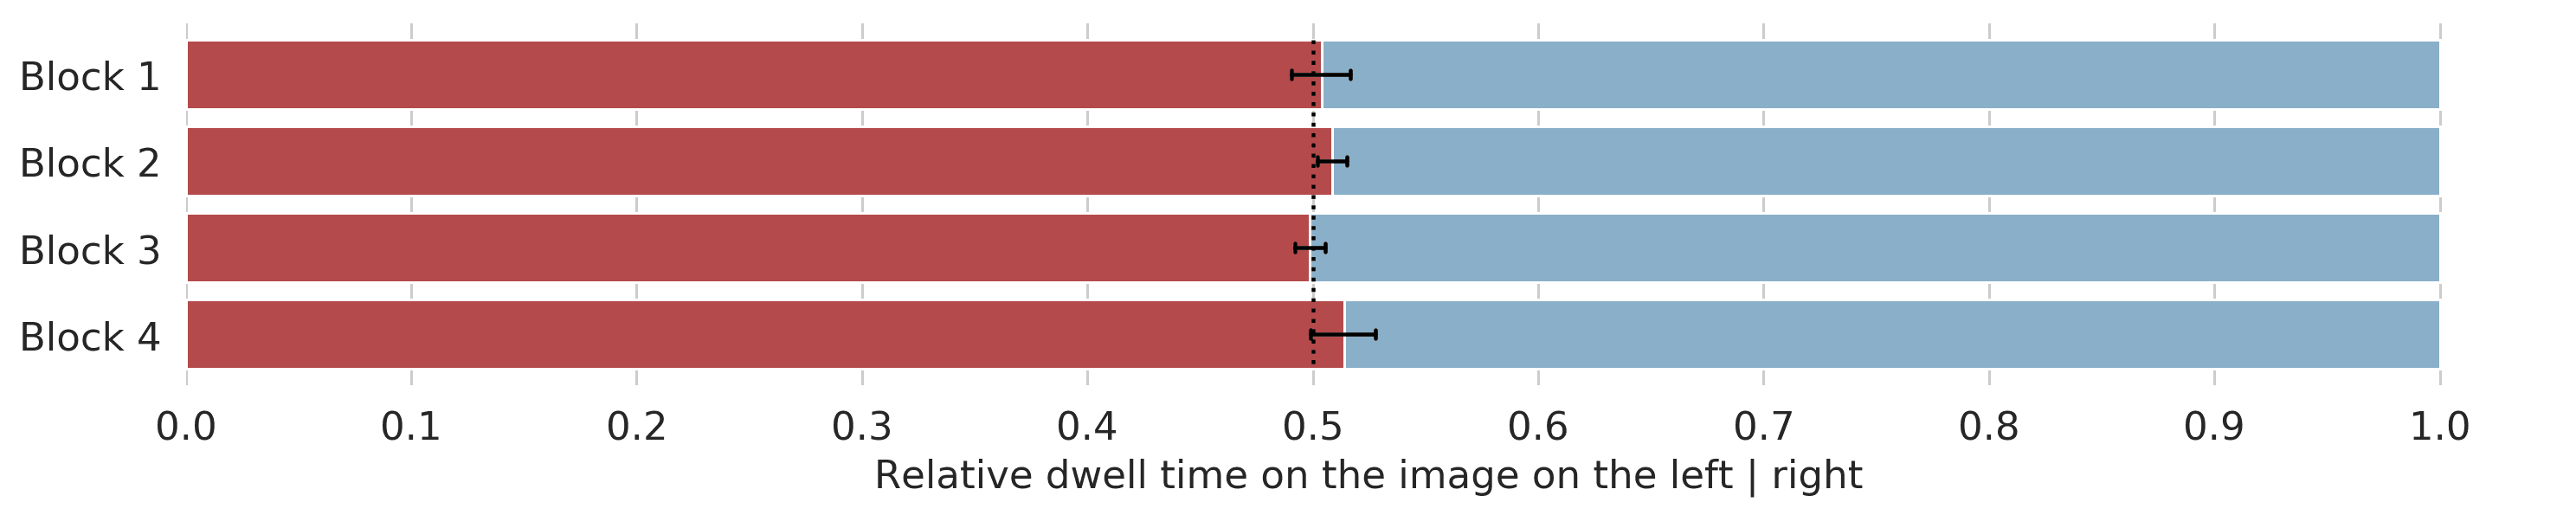
\includegraphics[width = \linewidth]{\imgpath/dwell_blocks.png}
  \caption{Exploration as measured by the relative dwell time on the left (red) and right (blue) images, at each block of the experimental session. Error bars depict the standard deviation of the mean.}
\label{fig:globsal-dwell_blocks}
\end{figure}

\begin{figure}[ht]
  \centering
  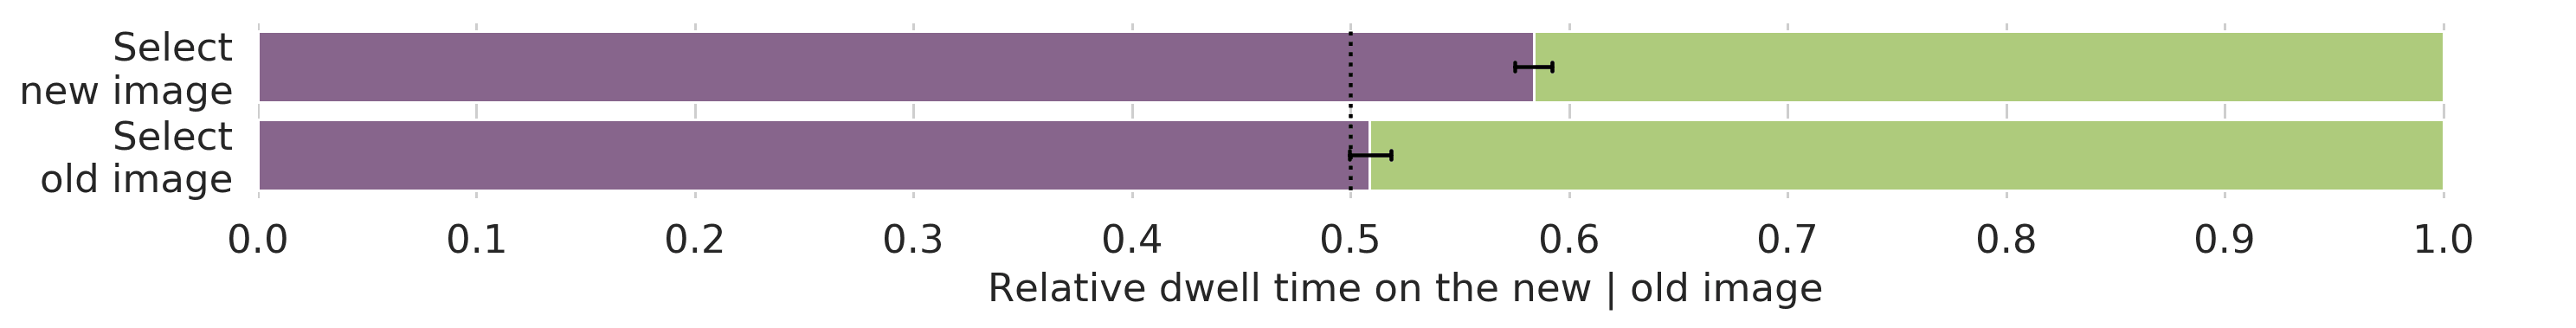
\includegraphics[width = \linewidth]{\imgpath/dwell_fam_task.png}
  \caption{Exploration as measured by the relative dwell time on the new (purple) and old (green) images, at blocks 2 and 3, where participants had the task of indicating the new and old image, respectively. Error bars depict the standard deviation of the mean.}
\label{fig:globsal-dwell_fam_task}
\end{figure}

For our main analysis regarding the interaction between exploration time and global image salience, we then contrasted the global salience score learned for each image with its respective dwell time averaged over all trials and subjects. The results revealed a significant positive correlation, indicating that images with larger global image salience led to a more intense exploration (Figure \ref{fig:globsal-dwell_scores}). Thus, global image salience describes not only a measure of which image attracts initial eye movements, but is also connected to longer exploration time, suggesting that global salience may describe the relative engagement of images. 

\begin{figure}[ht]
  \centering
  \begin{subfigure}{0.6 \linewidth}
      
\includegraphics[width = \linewidth]{\imgpath/legend_categories.png}
  \end{subfigure}
  \\
  \begin{subfigure}{0.6 \linewidth}
      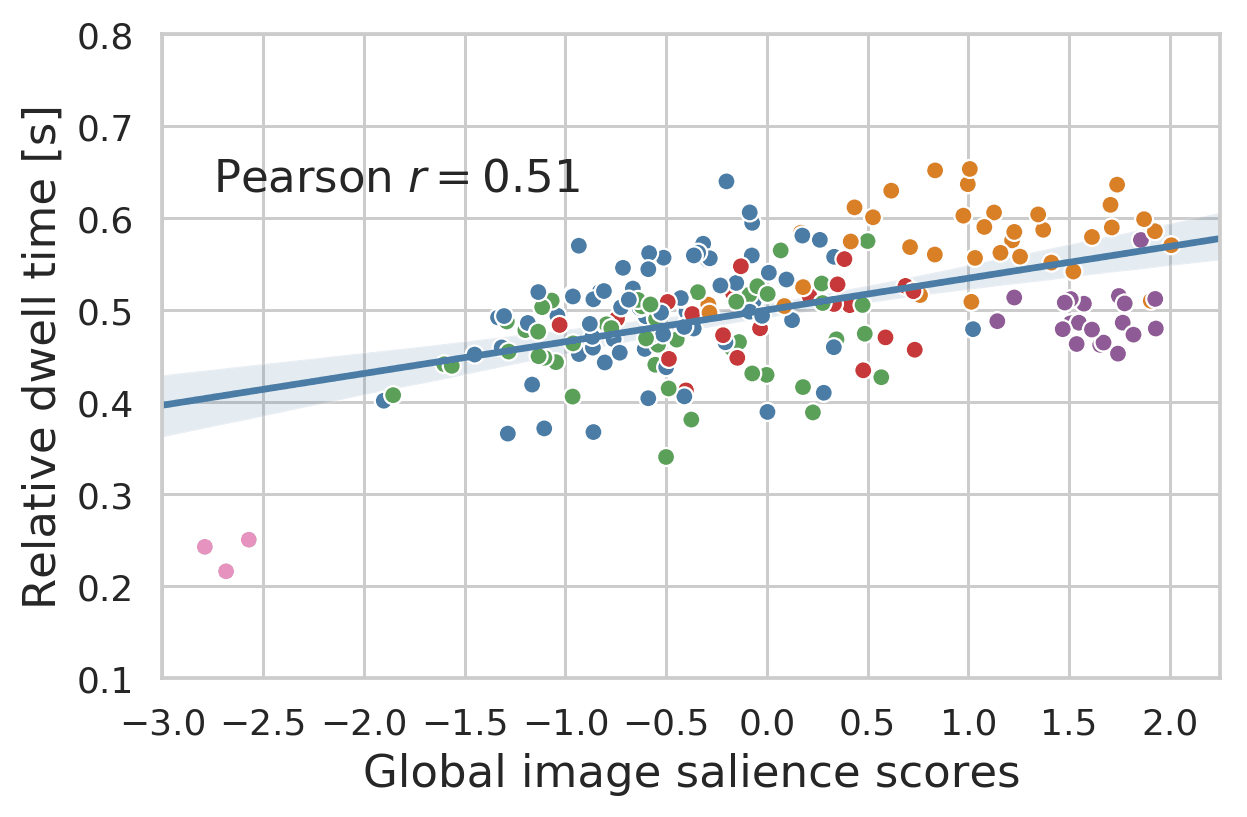
\includegraphics[width = \linewidth]{\imgpath/dwell_scores.png}
  \end{subfigure}
  \caption{Dwell time vs. global salience scores}
\label{fig:globsal-dwell_scores}
\end{figure}

Taken together, our results suggest that the task and familiarity---but not the spatial location of images---influenced the exploration time with respect to higher dwell times on unseen images in combination with the task to select the new image. Note, however, that regarding the effects of task our findings are restricted to the specific task assigned in our experiments, that is selecting which image is new or old. The effects of task in visual attention is an active field in visual perception and the results of multiple contributions should be taken together into consideration to draw robust conclusions. Finally, we also found that images with higher global salience correspondingly led to a larger time of exploration. These results fully support our fifth hypothesis.

\section{Discussion}
\label{sec:discussion}

We have presented a computational model trained on the saccadic behaviour of participants freely looking at pairs of competing stimuli, which is able to learn a robust score for each image, related to its likelihood of attracting the first fixation. This fully supports our first hypothesis and we refer to this property of natural images as the global visual salience.

The computational model consists of a logistic regression classifier, trained with the behavioural data of 49 participants who were presented 200 pairs of images. In order to reliably assess the performance of the model, we carried out a careful 25-fold cross-evaluation, with disjoint sets of participants for training, validating and testing. Given a pair of images from the set of 200, the model predicted the direction of the first saccade with 82 \% accuracy and 0.88 area under the ROC curve.

Throughout this chapter, we have analysed the general lateral bias towards the left image (H2), as well as other possible influences such as the familiarity with one of the images and the effect of a simple task (H3). Moreover, we have analysed the relationship of our proposed global salience with the local salience properties of the individual images (H4). Finally, we have also studied the total exploration time of each image in the eye-tracking experiment and compared it to the global salience, which is based upon the first fixation (H5).

Regarding the lateral bias, we found that participants tended to look more frequently towards the image on the left. Such left bias is typical in visual behaviour and has been found in many previous studies \citep{barton2006leftbias, guo2009leftbias, calenwalshe2014assymetricfixation, ossandon2014spatialbiases}. However, most of these studies presented only single images per stimulus. In this regard, it has been argued that cultural factors of the Western population who mostly take part in the research experiments may lead to a semantic processing of natural visual stimuli similar to the reading direction, that is from left to right \citep{spalek2005leftbias, zaeinab2016leftbias}.

In our study, about 63 \% of the first fixations landed on the left image. However, we also observed a high variability across participants, successfully captured by our computational model. In contrast, we showed that the given task in certain trials did not influence initial saccade behaviour. Participants equally distributed the target location of saccades on the presented images, regardless of familiarity and task relevance. Consequently, the spatial location of an image affected saccade behaviour, whereas the task as well as familiarity had no influence.

Importantly, we found that that global salience, that is the likelihood of an image attracting the first fixation when presented next another competing image, is independent of the low-level local salience properties of the respective images. The location of the first fixations made by the participants in the study did not correlate with the GBVS salience maps of the images and the saccadic choice---left or right---was neither explained by the GBVS salience mass difference. Hence, our results provide some new insights in the understanding of visual perception of natural images, showing that the global salience of an image is rather affected by the semantics of the content. For instance, images involving socially relevant content such as humans or faces led to higher global salience than images containing purely indoor, urban or natural scenes.

To gain further insight regarding this aspect, we computed the salience maps using Deep Gaze II \citep{kuemmerer2016deepgaze}, a computational salience model that is not limited to low-level features, but also makes use of high-level cues, obtained by pre-training the model with image object recognition tasks. We repeated the same analyses as with the GBVS model and we found that metrics derived from Deep Gaze salience maps did have a non-zero, yet moderate correlation with our proposed global salience. This, together with previous evidence about the importance of low- and high-level features in detecting fixations \citep{kuemmerer2017icfdeepgaze}, matches our finding that global salience cannot be explained by low-level properties of the images. However, the relatively low correlation further suggests that the initial preference for one of the images does not depend only on properties of the individual salience maps.

According to previous research, initial eye movements in young adults are based on bottom-up image features, whereas socially relevant content is fixated later in time \citep{acik2010bottomuptopdown}. Interestingly, as described above, we found that this was not the case when two images have been shown at the same time. Considering the very short reaction time between stimulus onset and the observers reaction to fixate one of the two images, it seems surprising that participants had to pre-scan both images in their peripheral visual field before initialising the first saccade. Thus, in contrast to classical salience maps, we might argue that the global salience of an image highly relates to the semantic and socially relevant content.

In order to further investigate the effects of the global image salience, we also evaluated the total time of image exploration, that is the dwell time. We hereby found that, different to the initial saccade, the spatial location of images did not affect the time participants explored the individual images of each image pair. However, the task and familiarity had an effect. We saw that in the task where participants had to select the new image, new images were explored longer than previously seen images. In contrast, the task asking to select the old image led to an almost equal exploration time on new and familiar images. Therefore, we conclude that participants in general tended to explore new images for a slightly longer time. Nevertheless and most importantly, we saw generally---and independent of the spatial location, task and familiarity---that images with higher global salience were explored longer in time. Thus, images with larger global salience did not only attract initial eye movements after stimulus onset, but also led to longer exploration times. These results support our assumption, that the global salience score of an image can also be interpreted as a measure of the general attraction of an image, in comparison to other images. 

In this regard, note that although we considered the location of the first fixation as the target variable to model the global salience scores and carry out the subsequent analyses, the same computational model and procedures can be used to model alternative aspects of the behavioural responses. For instance, the model could be trained to fit the dwell time---which we have found to be positively correlated with the global salience based on the first fixations---, the engagement---time until fixating away---or the number of saccades.

In spite of the high performance of our computational model and its potential to assign reliable global salience scores to natural images, an important limitation is that the model and thus the scores are dependent on the image set that we used. Whereas local salience maps rely on image features, our proposed global salience model relies on the differences between the stimuli and the behavioural differences that they elicit on the participants. We observed significant differences between image categories, for example humans versus indoor scenes, but this is only one initial step and future work should investigate what other factors influence the global image salience. For example, it would be interesting to train a deep neural network with a possibly larger  set of images and the global salience scores learned by our model as labels, similarly to how Deep Gaze was trained to predict fixation locations. This could shed more light on what features make an image more globally salient.

Another related, interesting avenue for future work is investigating the global salience in homogeneous data sets, that is with images of similar content. Our work has shown that large differences exist between images with somehow different content, for instance containing humans or not. However, we did not observe significantly difference global salience between natural and urban scenes (see Figure~\ref{fig:globsal-global_salience_categories}), although significant difference do exist between specific images. An interesting question is: \textit{what} makes one image more likely to attract the first fixation, when presented alongside a semantically similar image? We think an answer to this question can be sought by combining a similar experimental setup as the one presented in this work, with additional data, and making use of advanced feature analysis, such as deep artificial neural networks, as mentioned above.

For instance, small changes in the context information of single images, might already have a dramatic influence on reaction times in decision tasks \citep{kietzmann2015topdown}. In addition, the global salience was based on eye movement behaviour of human data. Depending on the choice of participants, e.g. different culture, age, personal interests and emotions, our model could have revealed different results \citep{balcetis2006topdown, dowiasch2015aging}. Again, further studies might use the model on a wider range of participants, in order to validate the specific global salience and thus attraction of images. 

In contrast, differences in the global salience between participant groups could be a great advantage in certain research fields. In medical applications for instance, researchers could identify specific diseases, such autistic spectrum disorder (ASD). In such example, our method could generate a model of the global visual salience of both control people and individuals with certain condition, and then be used for diagnosis. Another use case of our model would be marketing research, where the attraction of different images could be compared adequately based on intuitive visual behaviour. Thus, depending on the research question, the global image salience might provide a new insight in prediction and analysis of visual behaviour.

\section{Conclusion}
\label{sec:conclusion}

Previous research has investigated the local salience properties of single images, which has helped understand visual behaviour. However, assigning a single and unique global salience score to an image as a whole has been neglected. Here, we thus trained a logistic regression model to learn unique, global salience scores for each tested image. We hereby showed that images can indeed be ranked according to their global salience, providing a new method to predict eye movement behaviour across images with distinct semantic content. These results could be used in a variety of research, such as medicine or marketing.

\chapterbibliography
}
